\chapter{Experiment}
\section{System}
\subsection{Hardware}
The end system has two arrays, each with three microphones mounted on the vertices of a $20$ cm equilateral triangle. We used omni-directional foil electret condenser microphone due to its low cost and small size. The microphone has a frequency range of $100$ to $10K$ Hz, and a minimum SNR of 58dB\cite{sys:1}. We also used operational amplifer OPA344 from Texas Instrument to amplify the microphone output by a factor of 100, so the received signal can be easily picked up by the analog-to-digital converter (ADC) module installed on the micro-controller. The micro-controller board used in this project is \emph{teensy 3.1}, and it is attached to one of the vertices of the triangle. Fig~\ref{fig:setup_array} shows a picture of the array setup.  The micro-controller contains an onboard RAM of $64$k, and an ADC module capable of sampling at $500$kHz~\cite{tdoa:micloc, sys:teensy}. In this project, the micro-controller collects microphone data on all three channels for a duration $12$ milliseconds and then sends the recorded data to a computer through the USB port for localization. 

\begin{figure}[h!]
  \centering
  \begin{subfigure}[]{.48\textwidth}
    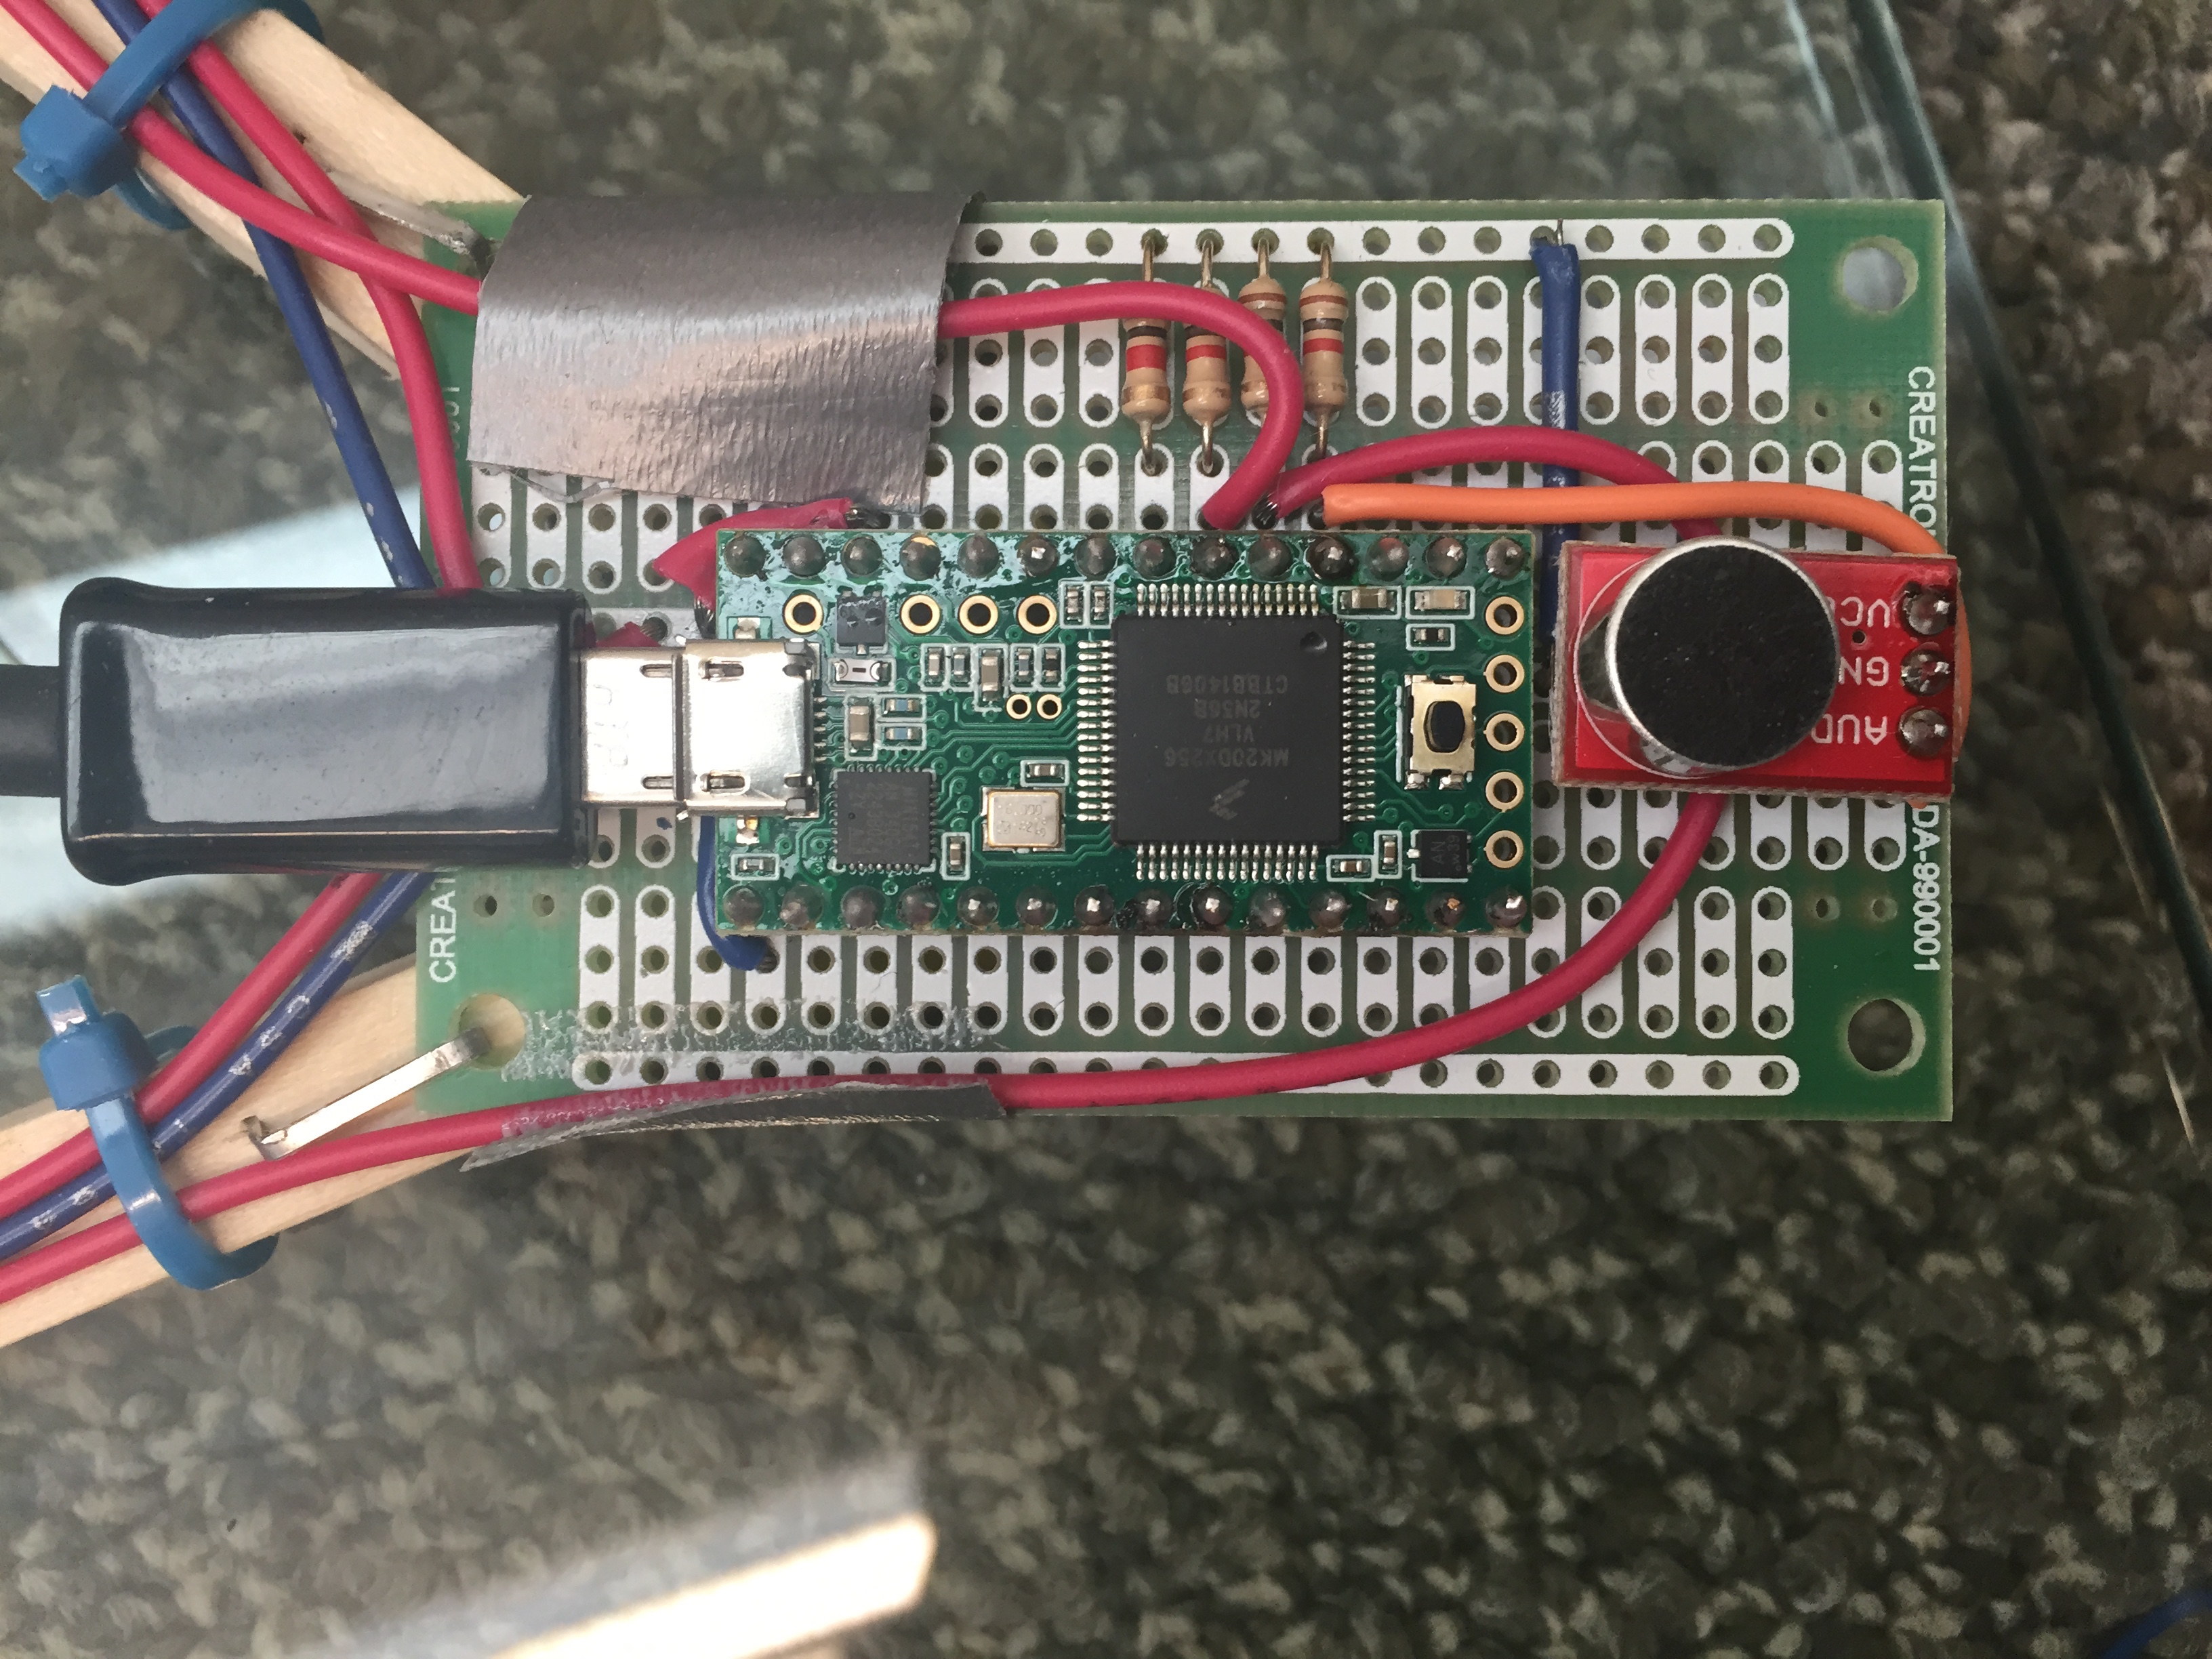
\includegraphics[width=\textwidth]{array_close.JPG}
    \caption{micro-controller}
  \end{subfigure}
  \begin{subfigure}[]{.48\textwidth}
    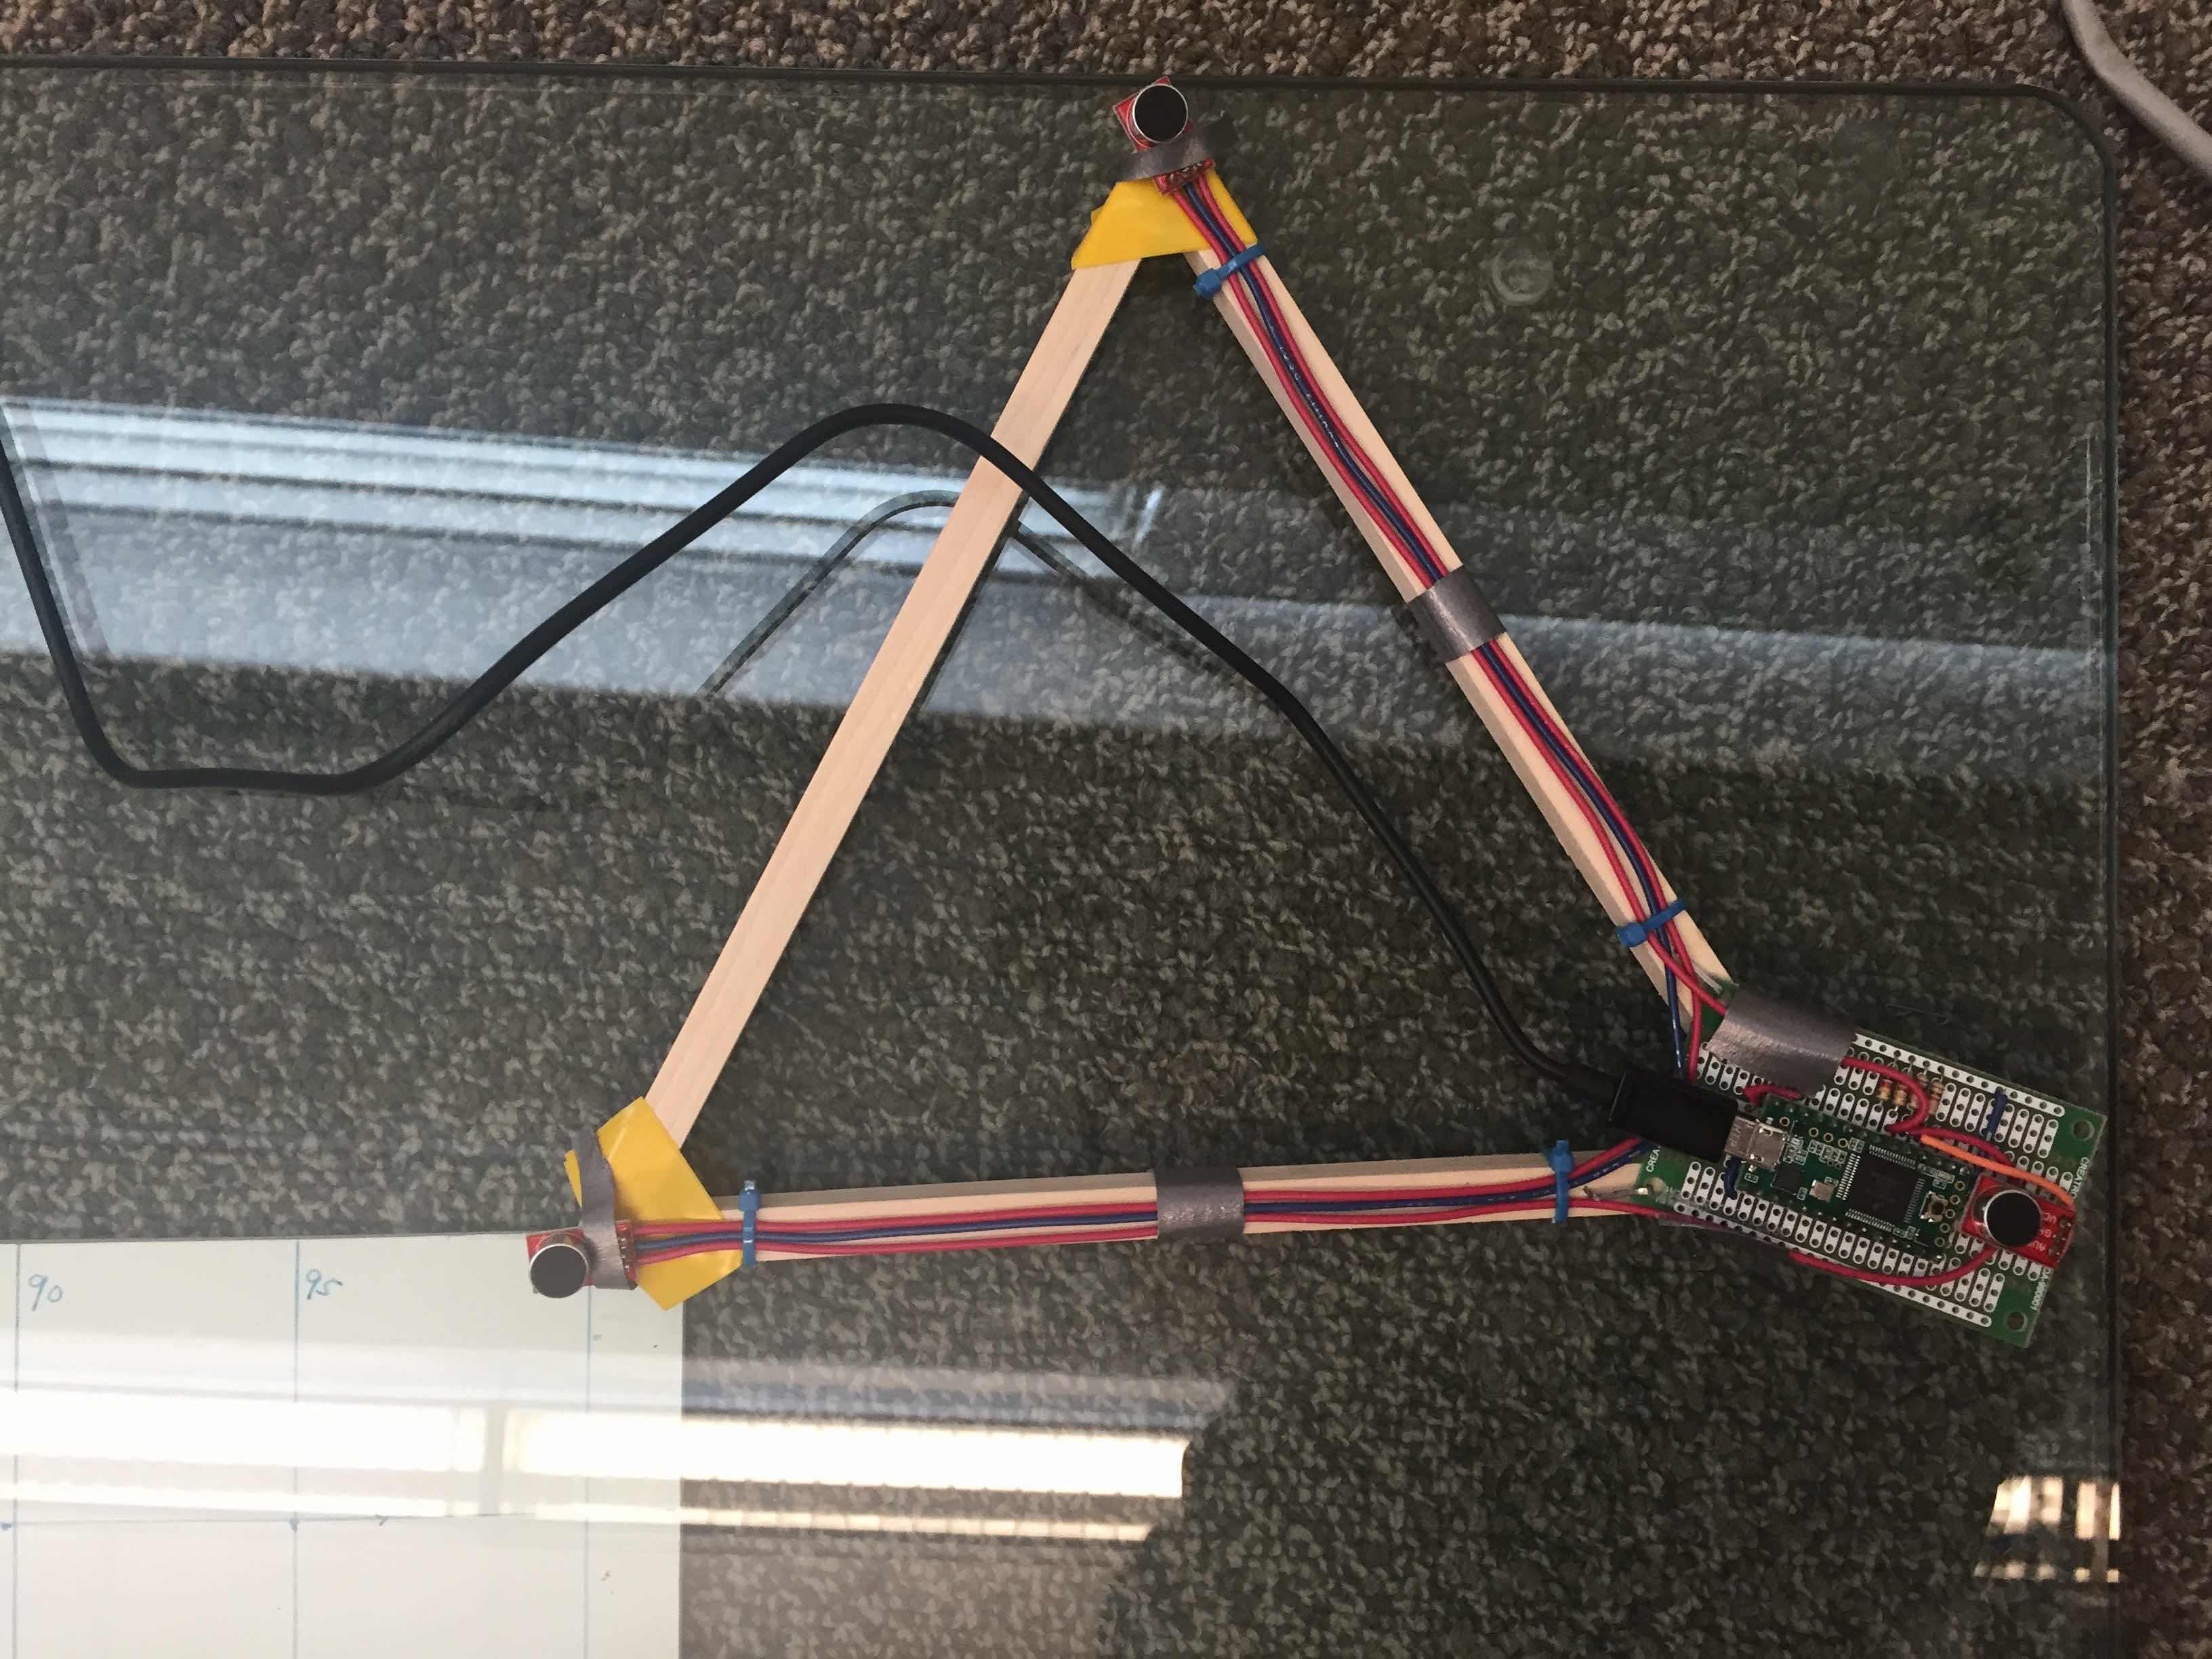
\includegraphics[width=\textwidth]{array.JPG}
    \caption{array}
  \end{subfigure}
  \begin{subfigure}[]{.48\textwidth}
    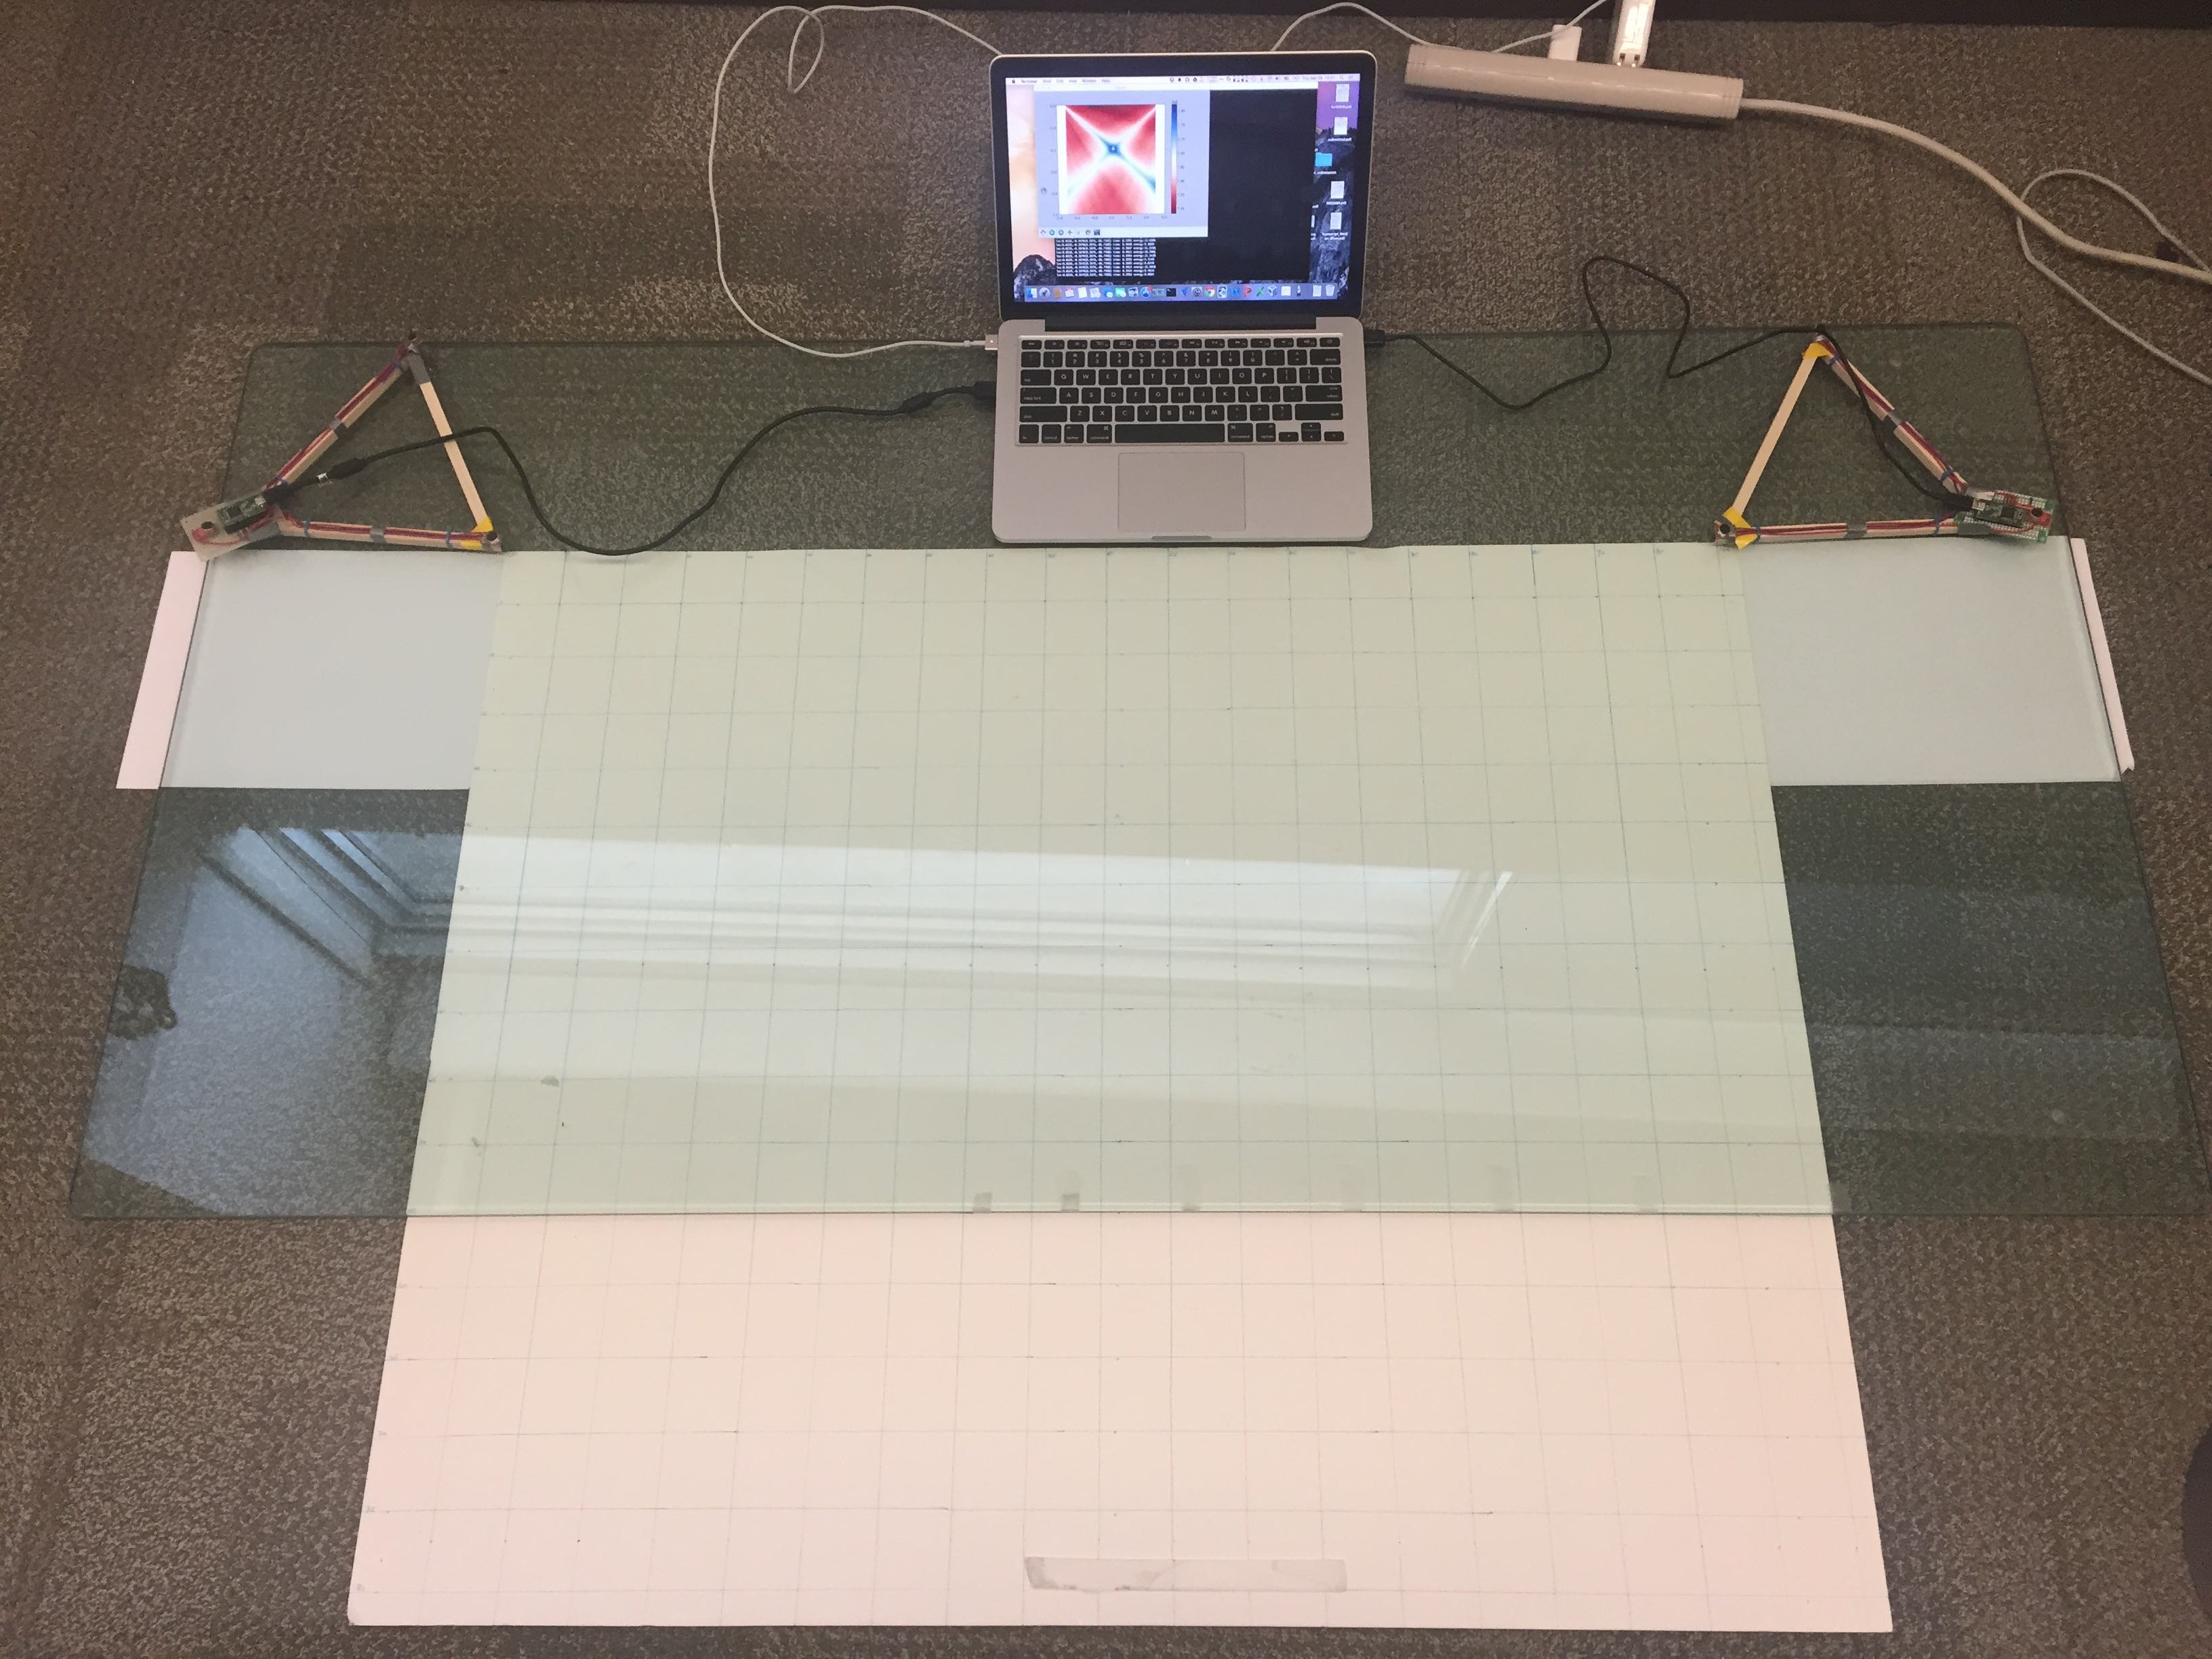
\includegraphics[width=\textwidth]{setup_2.JPG}
    \caption{two arrays}
  \end{subfigure}
  \caption{Localization system setup}
  \label{fig:setup_array}
\end{figure}

\subsection{Software}

On the software side, \emph{Python} is used as the main programming language since it has extensive libraries in both real time data handling and signal processing. \emph{ZeroMQ} is an inter process messaging queue that is used in our system to pass data across different modules. Our system is made up of two data acquisition modules (each is used to receive raw date from microphone array output) and one localization module (listens to both data acquisition modules and perform localization using the raw microphone data). Using ZeroMQ as connections to different modules adds flexibility to our system, as we can design applications such as the drawing application we have used in our system to interface only with the localization module and disregard how the microphone data is collected. Other localization applications can be easily integrated into our system by connecting them with the localization module. Furthermore, we have built a recording module that interfaces with the data acquisition modules for offline analysis and parameter tuning. 

To handle the uncertainty in TDOA estimation, instead of using point estimate that maximizes equation~\ref{eq:gcc}, we take the cross-correlation output(equation~\ref{eq:gcc2}) as a measure of the likelihood of different arrival time differences. Each index $i$ from the cross-correlation vector denotes the time delay across the two microphones receiving the acoustic signal, and the cross-correlation value $k$[i] at each index $i$ denotes the likelihood of the time delay being $i$. 

For each microphone array, we build a heatmap of likelihood for the region. The intensity at each point on the heatmap represents the likelihood of it being the source. To generate the likelihood heatmap for an microphone array, we apply the following algorithm. For each point ($x$,$y$) on the grid, the theoretical TDOA to each microphone pair can be precomputed using:
\[
 D_{m_1,m_2}(x,y) =  \frac{((x-x_1)^2 + (y-y_1)^2)^{0.5} - ((x-x_2)^2 + (y-y_2)^2)^{0.5}}{v}
\]
where ($x_1, y_1$) and ($x_2, y_2$) are the locations of the microphone pair and $v$ is the speed of sound. Then the heatmap can be generated by going through all the points on the grid and performing a lookup using equation~\ref{eq:gcc2}. With three microphones $m_1,m_2,$ and $m_3$, there are three microphone pairs: $m_1m_2,m_1m_3,$ and $m_2m_3$. The theoretical TDOA from each location $(x,y)$ to each microphone pair is precomputed and stored in $D_{m_1,m_2}(x,y)$, $D_{m_1,m_3}(x,y)$, and $D_{m_2,m_3}(x,y)$. Then the likelihood map $L(x,y)$ can be built by superposing the likelihood from each microphone pair:
\begin{eqnarray*}
L(x,y) &=& R_{m_1,m_2}(D_{m_1,m_2}(x,y)) + R_{m_1,m_3}(D_{m_1,m_3}(x,y)) \\
 & & +R_{m_2,m_3}(D_{m_2,m_3}(x,y)) 
\end{eqnarray*}
where $R_{m_1,m_2}(\tau)$,$R_{m_1,m_3}(\tau)$, and $R_{m_2,m_3}(\tau)$ denote GCC output from microphone pairs $m_1m_2,m_1m_3,$ and $m_2m_3$.

Likelihood maps from two arrays can be combined into the final likelihood map:
\begin{equation}\label{eq:combine_l}
L(x,y) = L_1(x,y) L_2(x,y)
\end{equation}
where $L_1(x,y)$ and $L_2(x,y)$ represent the likelihood map from array $1$ and array $2$.

\begin{figure}[h!]
  \centering
  \begin{subfigure}[]{.48\textwidth}
    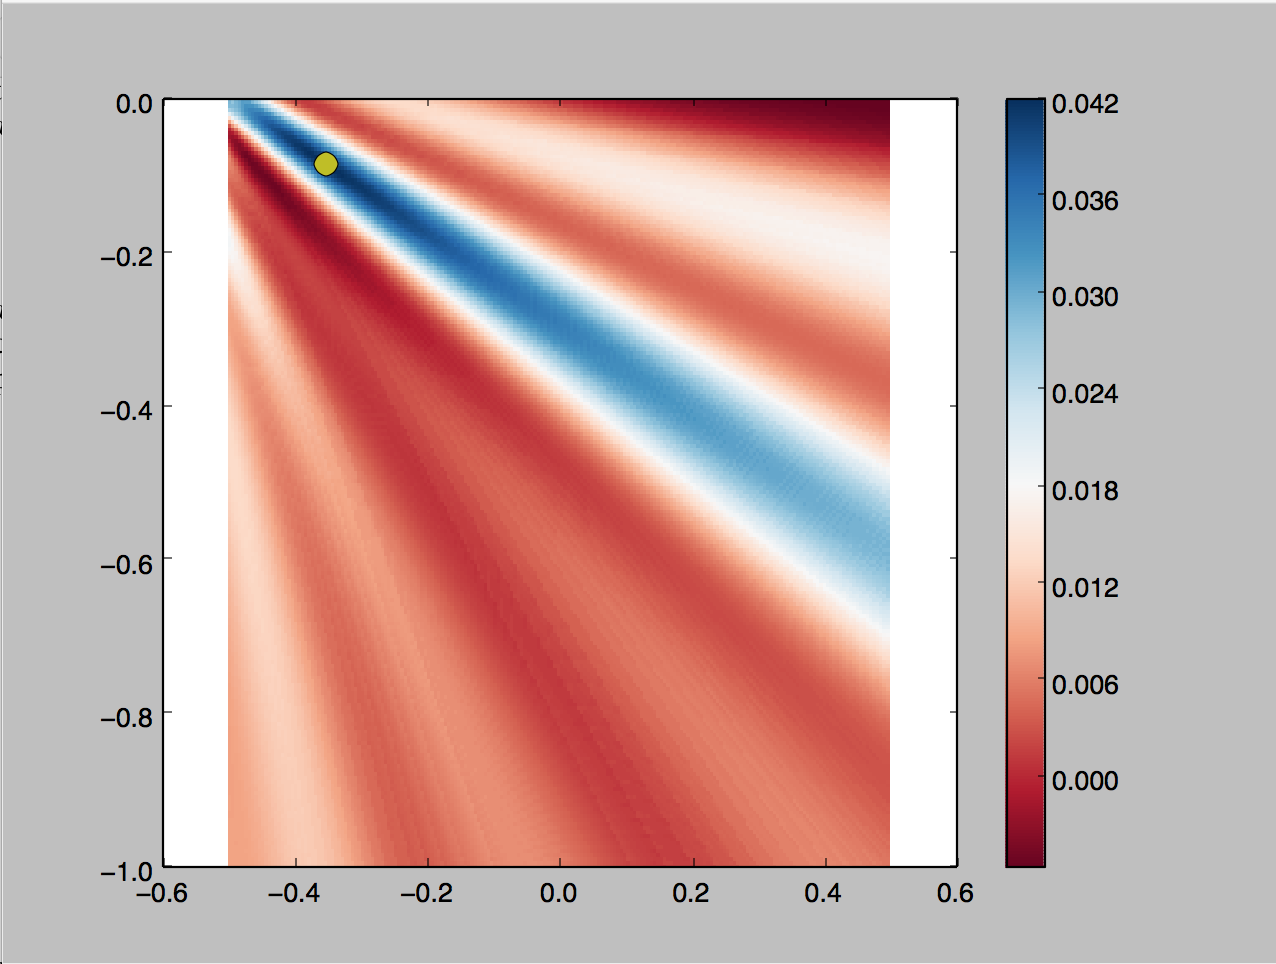
\includegraphics[width=\textwidth]{left.png}
    \caption{localization with only array 1}
    \label{fig:liklihood1}
  \end{subfigure}
  \begin{subfigure}[]{.48\textwidth}
    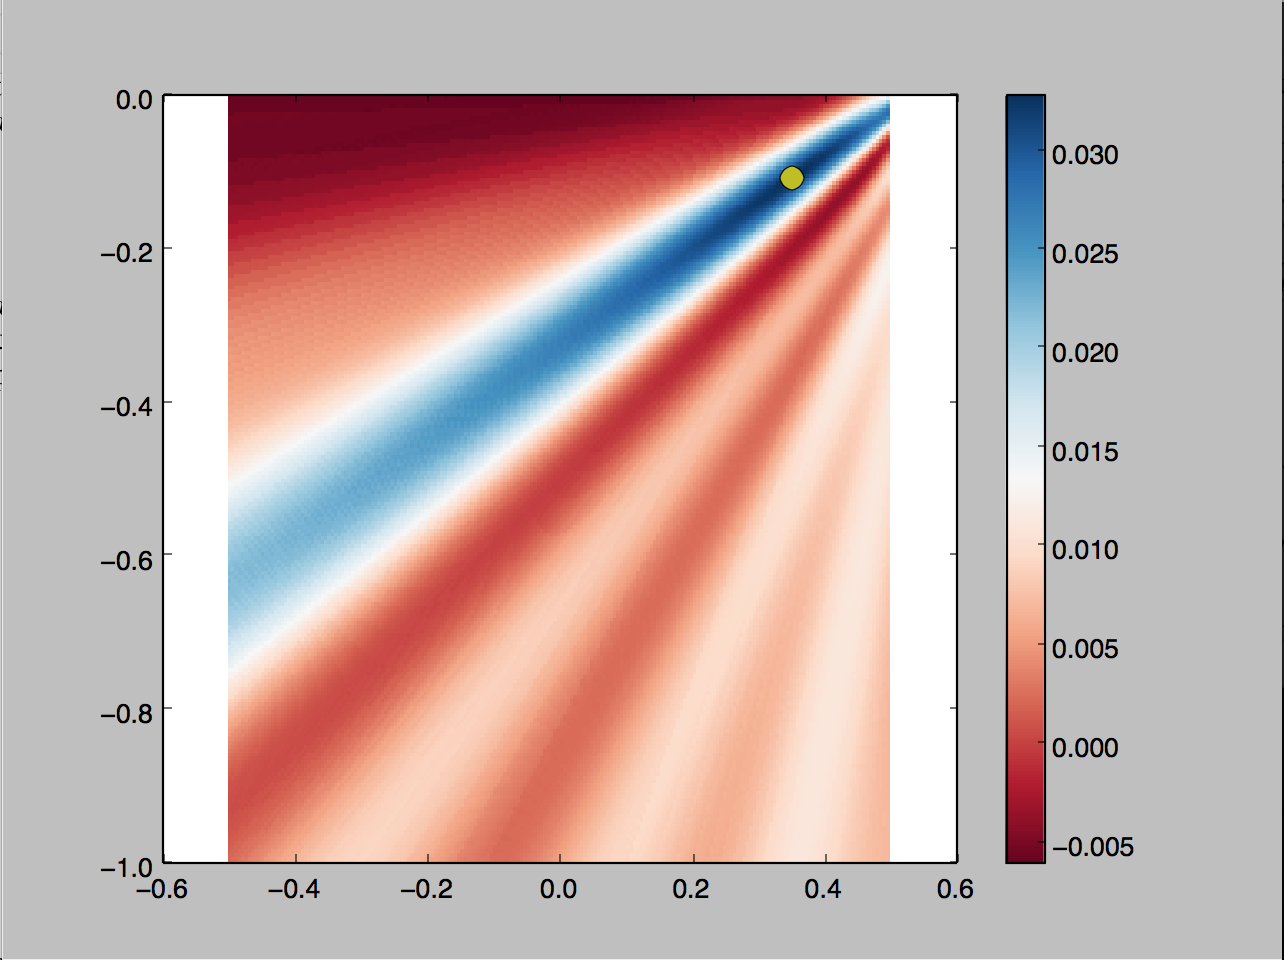
\includegraphics[width=\textwidth]{right.png}
    \caption{localization with only array 2}
    \label{fig:liklihood2}
  \end{subfigure}
  \begin{subfigure}[]{.48\textwidth}
    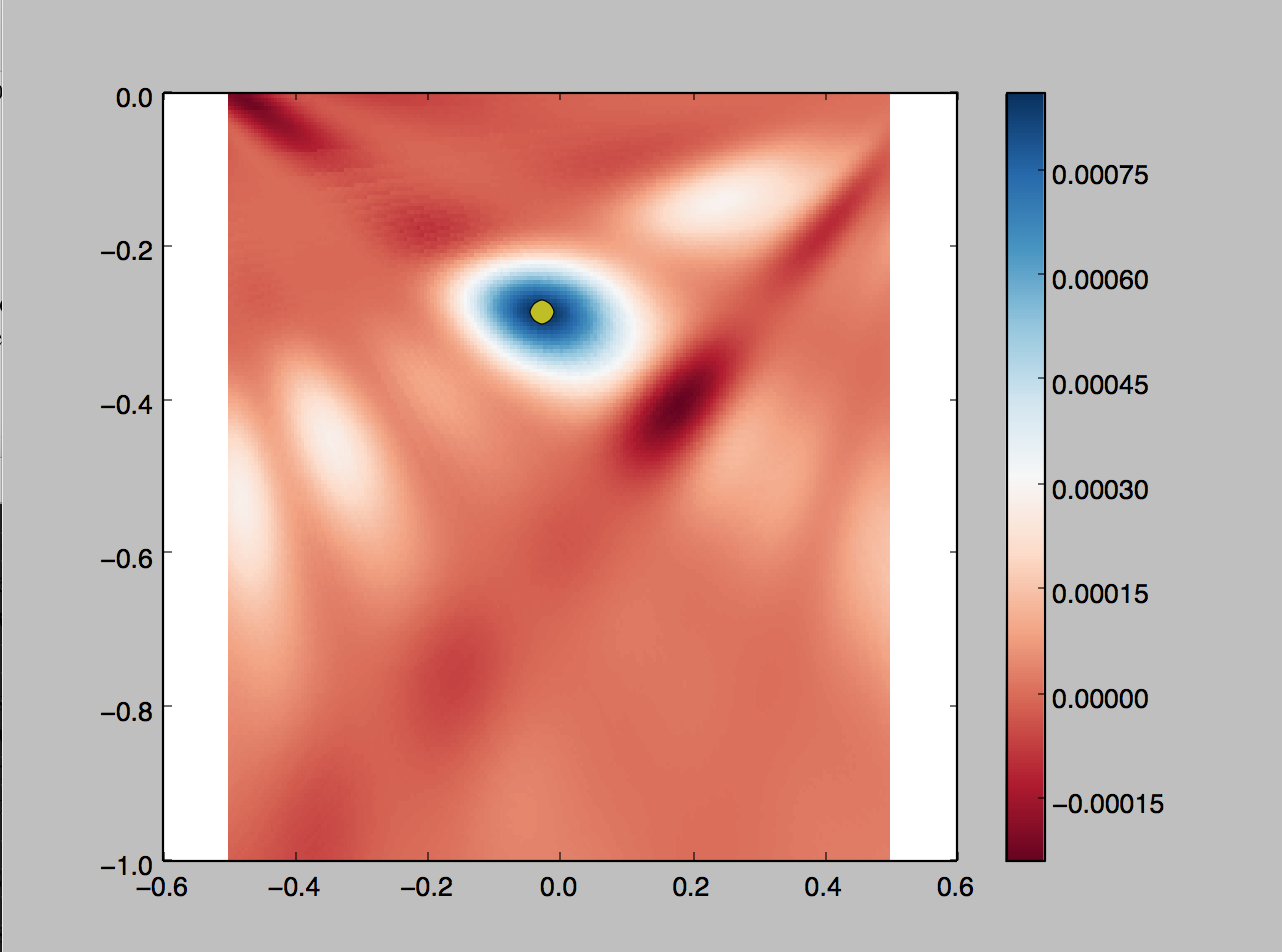
\includegraphics[width=\textwidth]{combined.png}
    \caption{localization with both arrays}
    \label{fig:liklihood3}
  \end{subfigure}
  \caption{Likelihood maps for localization. The source is placed at $(0.0,-0.3)$ m}
  \label{fig:liklihood}
\end{figure}

To see the effect of accuracy improvement using multiple arrays, fig~\ref{fig:liklihood} shows a real life localization where the source is placed at $(0$ cm$,-30$ cm$)$. The top two figures show the individual likelihood maps produced by single microphone arrays. We can see that the individual arrays can give accurate angle estimate, but have high uncertainty in distance estimate. The bottom figure shows the combined likelihood map according to equation~\ref{eq:combine_l}. The combined likelihood map demonstrated that by merging estimates from two arrays the system is able to perform more accurate localization. 


From a timing point of view, the micro-controller spends $12$ milliseconds on sampling the microphone data before sending it to a computer for processing. Sending the data through the USB port takes another $15$ milliseconds, and processing on the computer takes around $50$ milliseconds. Therefore, the total time lag between sound source and localization is around $80$ milliseconds.

\clearpage

\section{Setup}

We conducted two sets of experiments to evaluate the system's localization accuracy: one on point localization and the other on movement tracking. For the point localization experiment we looked into using different window size of audio signals and different prefiltering methods. The size of the window limits how far apart the microphone arrays can be. If the time delay from one microphone array to another exceeds the size of the window, the location of the source can never be estimated. A large window size gives a more complete acoustic signal which makes cross-correlation less prone to noise. However, the larger the window size the more time it takes to compute the cross-correlation. This is a trade off that we will address.  

For the movement tracking experiment, on top of the varying window size, we also looked into varying the movement speed of the audio source, applying different movement filters, and using different types of audio source. By applying an increasing movement speed of the audio source, we can test how fast the system can track an audible object moving in real time. We experimented with two types of music as our audio source for movement tracking, one with no low volume throughout, and the other with intermittent low or no volume. We want to test how the system performs when the audio source isn't continuously outputting sound. Furthermore, we applied different movement filters to help reduce noise and smooth out the path of the moving audio source.  

\subsection{Point localization}

\begin{figure}[h!]
  \centering
  \begin{subfigure}[]{.48\textwidth}
    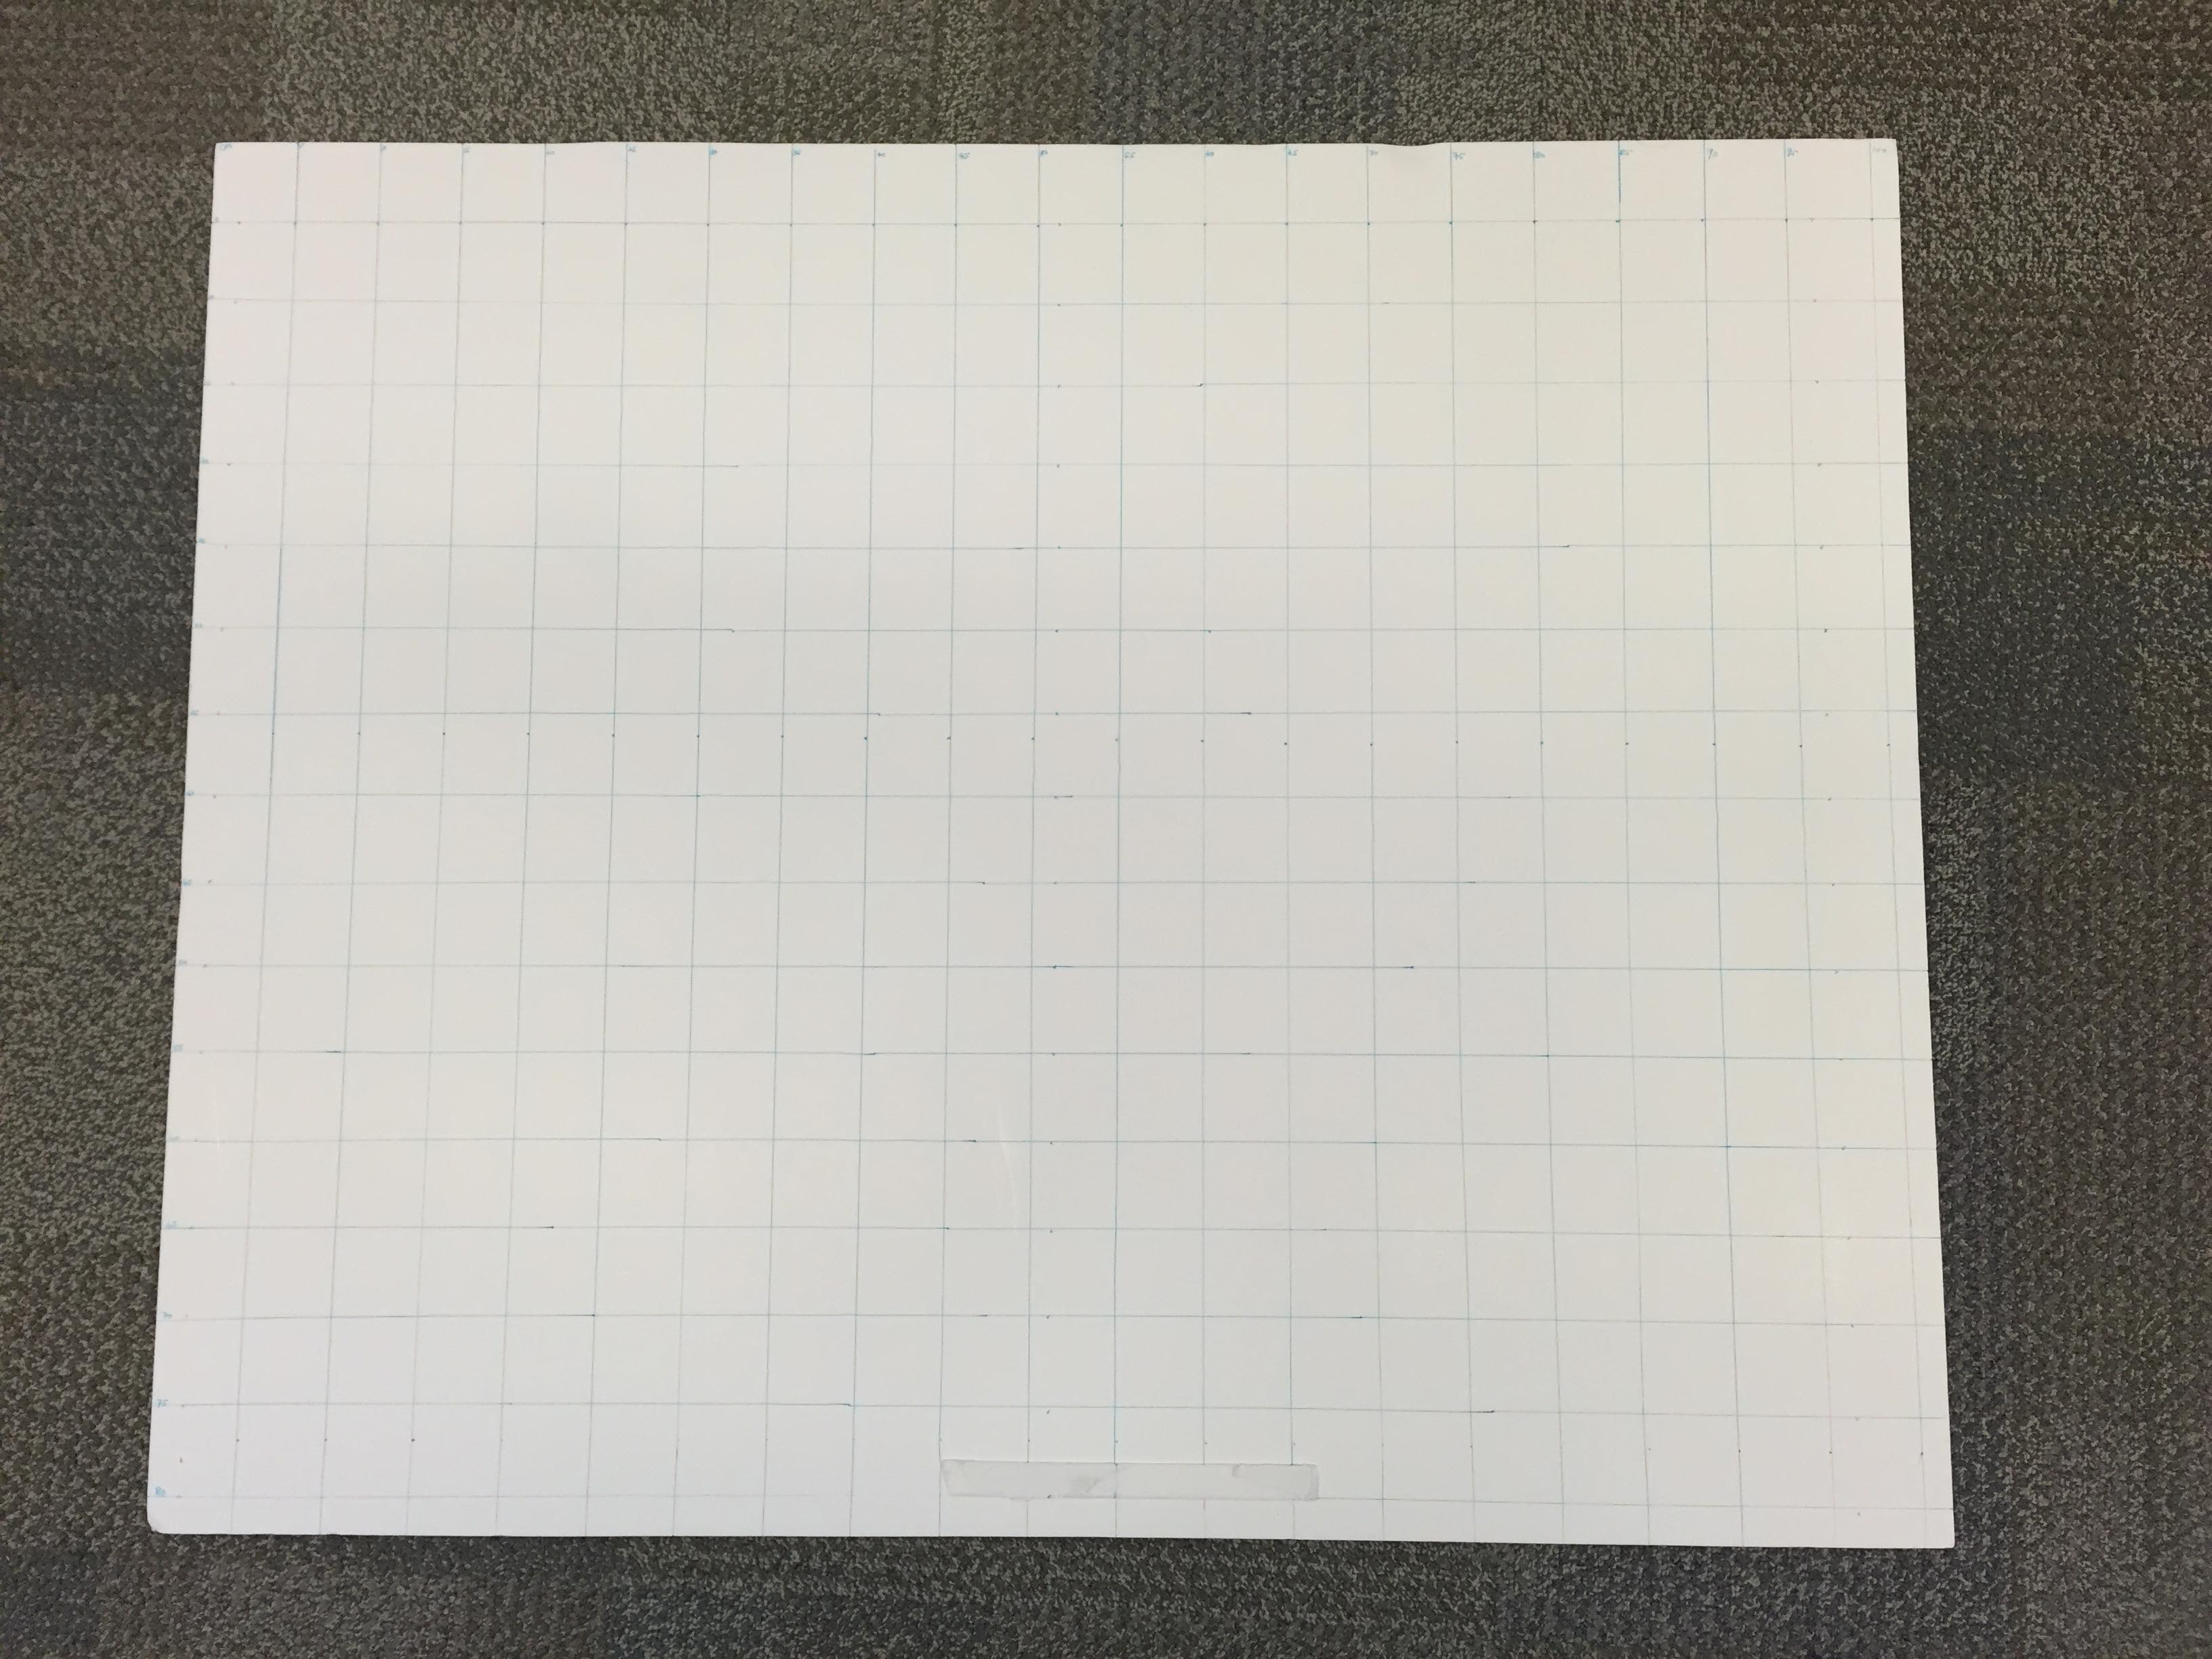
\includegraphics[width=\textwidth]{setup_1.JPG}
    \caption{1 meter by 1 meter grid}
  \end{subfigure}
  \begin{subfigure}[]{.48\textwidth}
    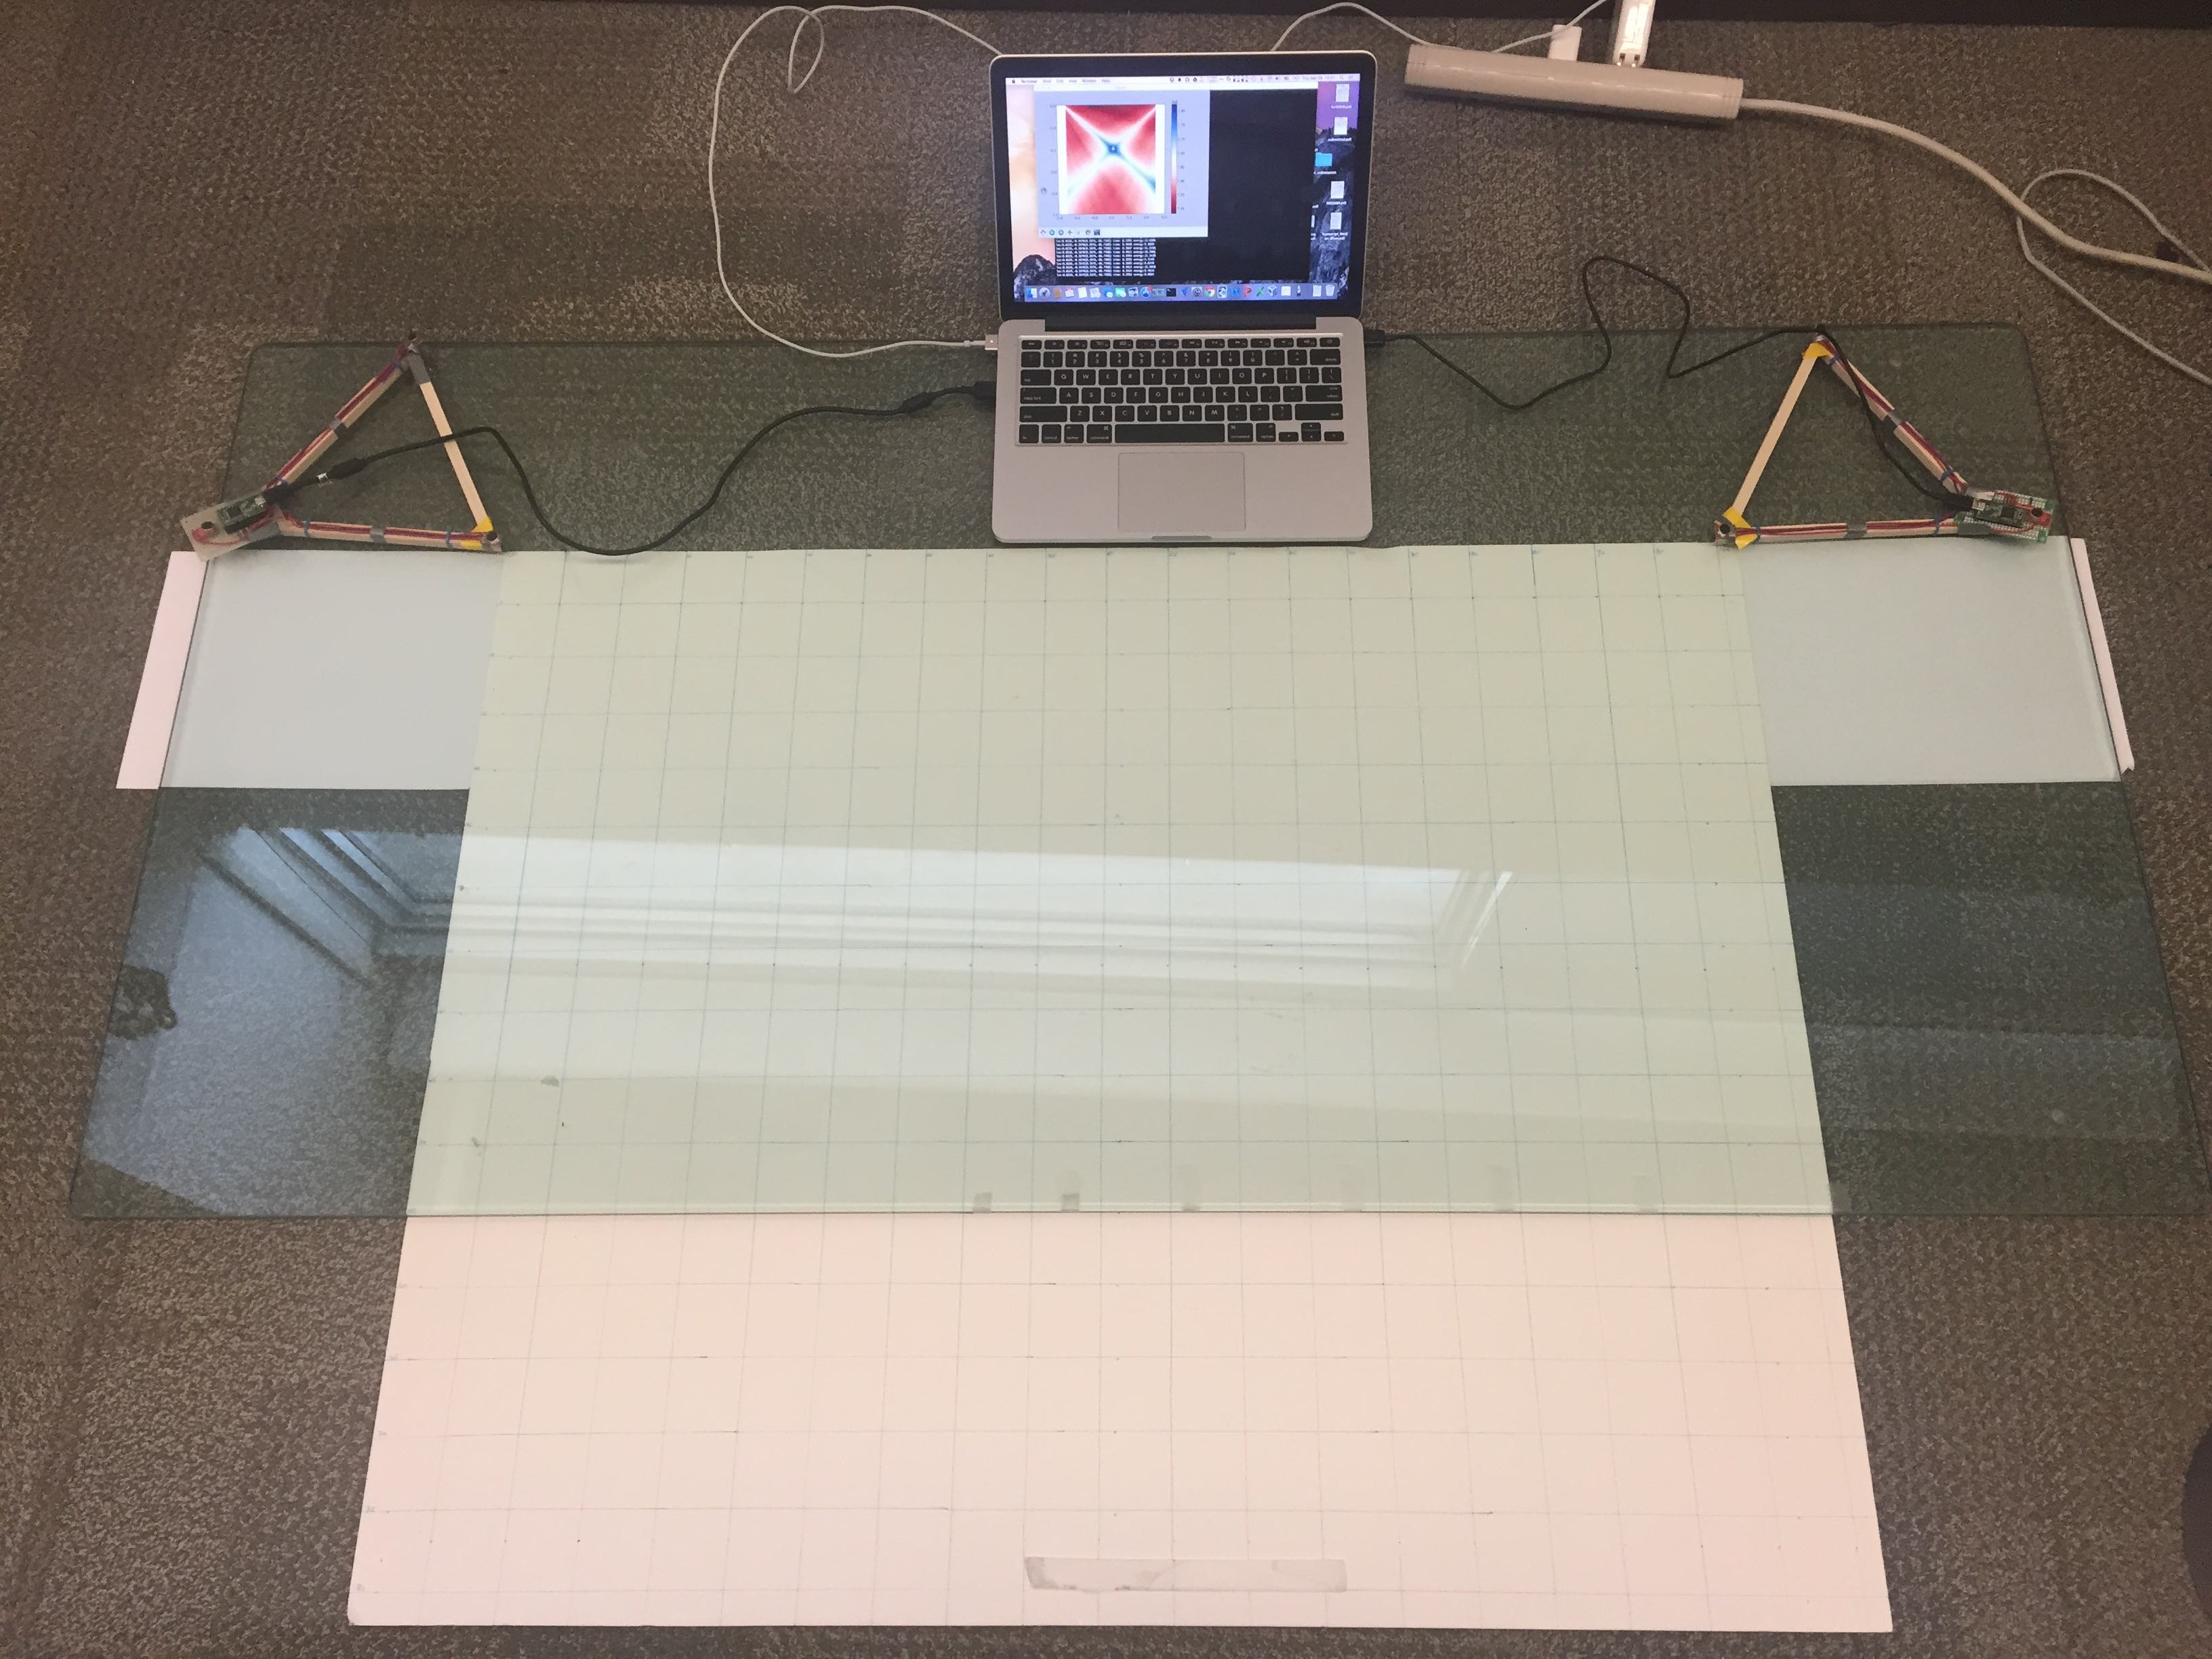
\includegraphics[width=\textwidth]{setup_2.JPG}
    \caption{array placement}
  \end{subfigure}
  \caption{Setup for point localization evaluation}
  \label{fig:setup_point}
\end{figure}

An one meter by one meter grid was set up where the arrays were placed at the top left and top right corners of the grid. Fig~\ref{fig:setup_point} shows a picture of the setup. A total of $32$ testing locations were chosen uniformly in this grid. Testing is done by placing the audio source at each grid location, and turning on the audio source with white noise. We reported the error as the average distance between our placement of the audio source and the location estimated from the arrays.

\subsection{Movement tracking}

\begin{figure}[h!]
  \centering
%  \begin{subfigure}[]{.2\textwidth}
%    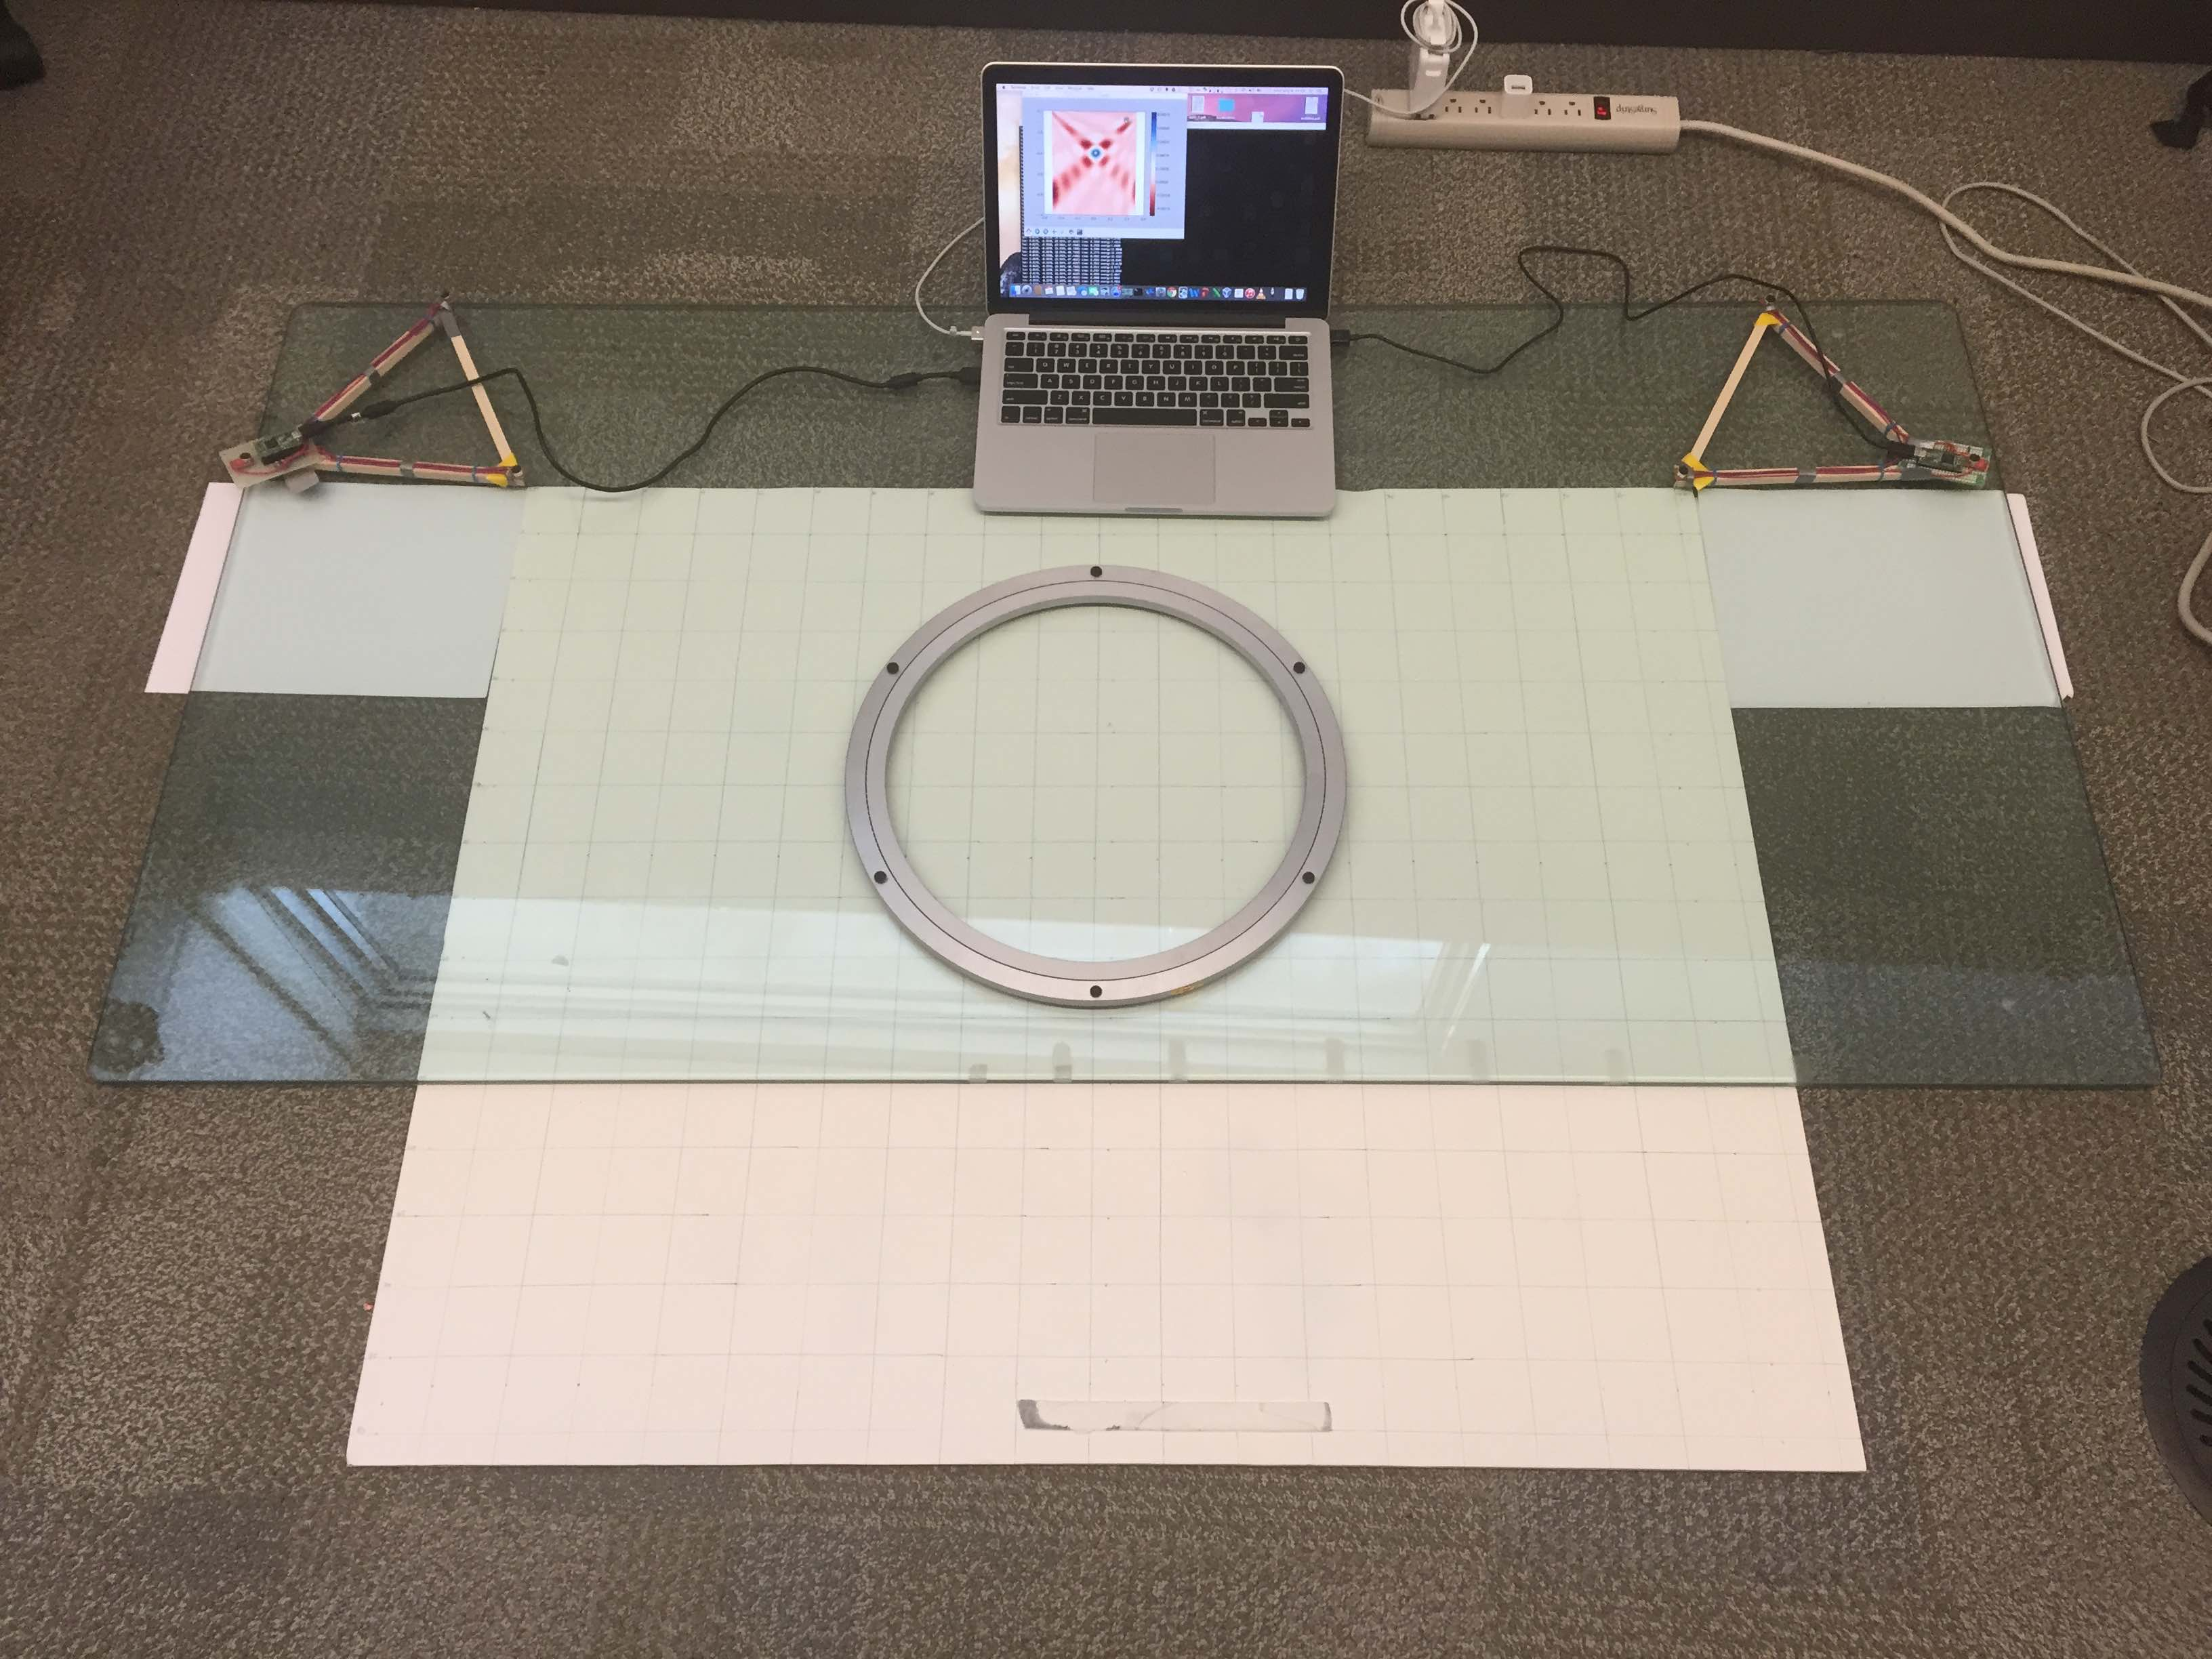
\includegraphics[width=\textwidth]{setup_ring.JPG}
%  \end{subfigure}
  \begin{subfigure}[]{1.0\textwidth}
    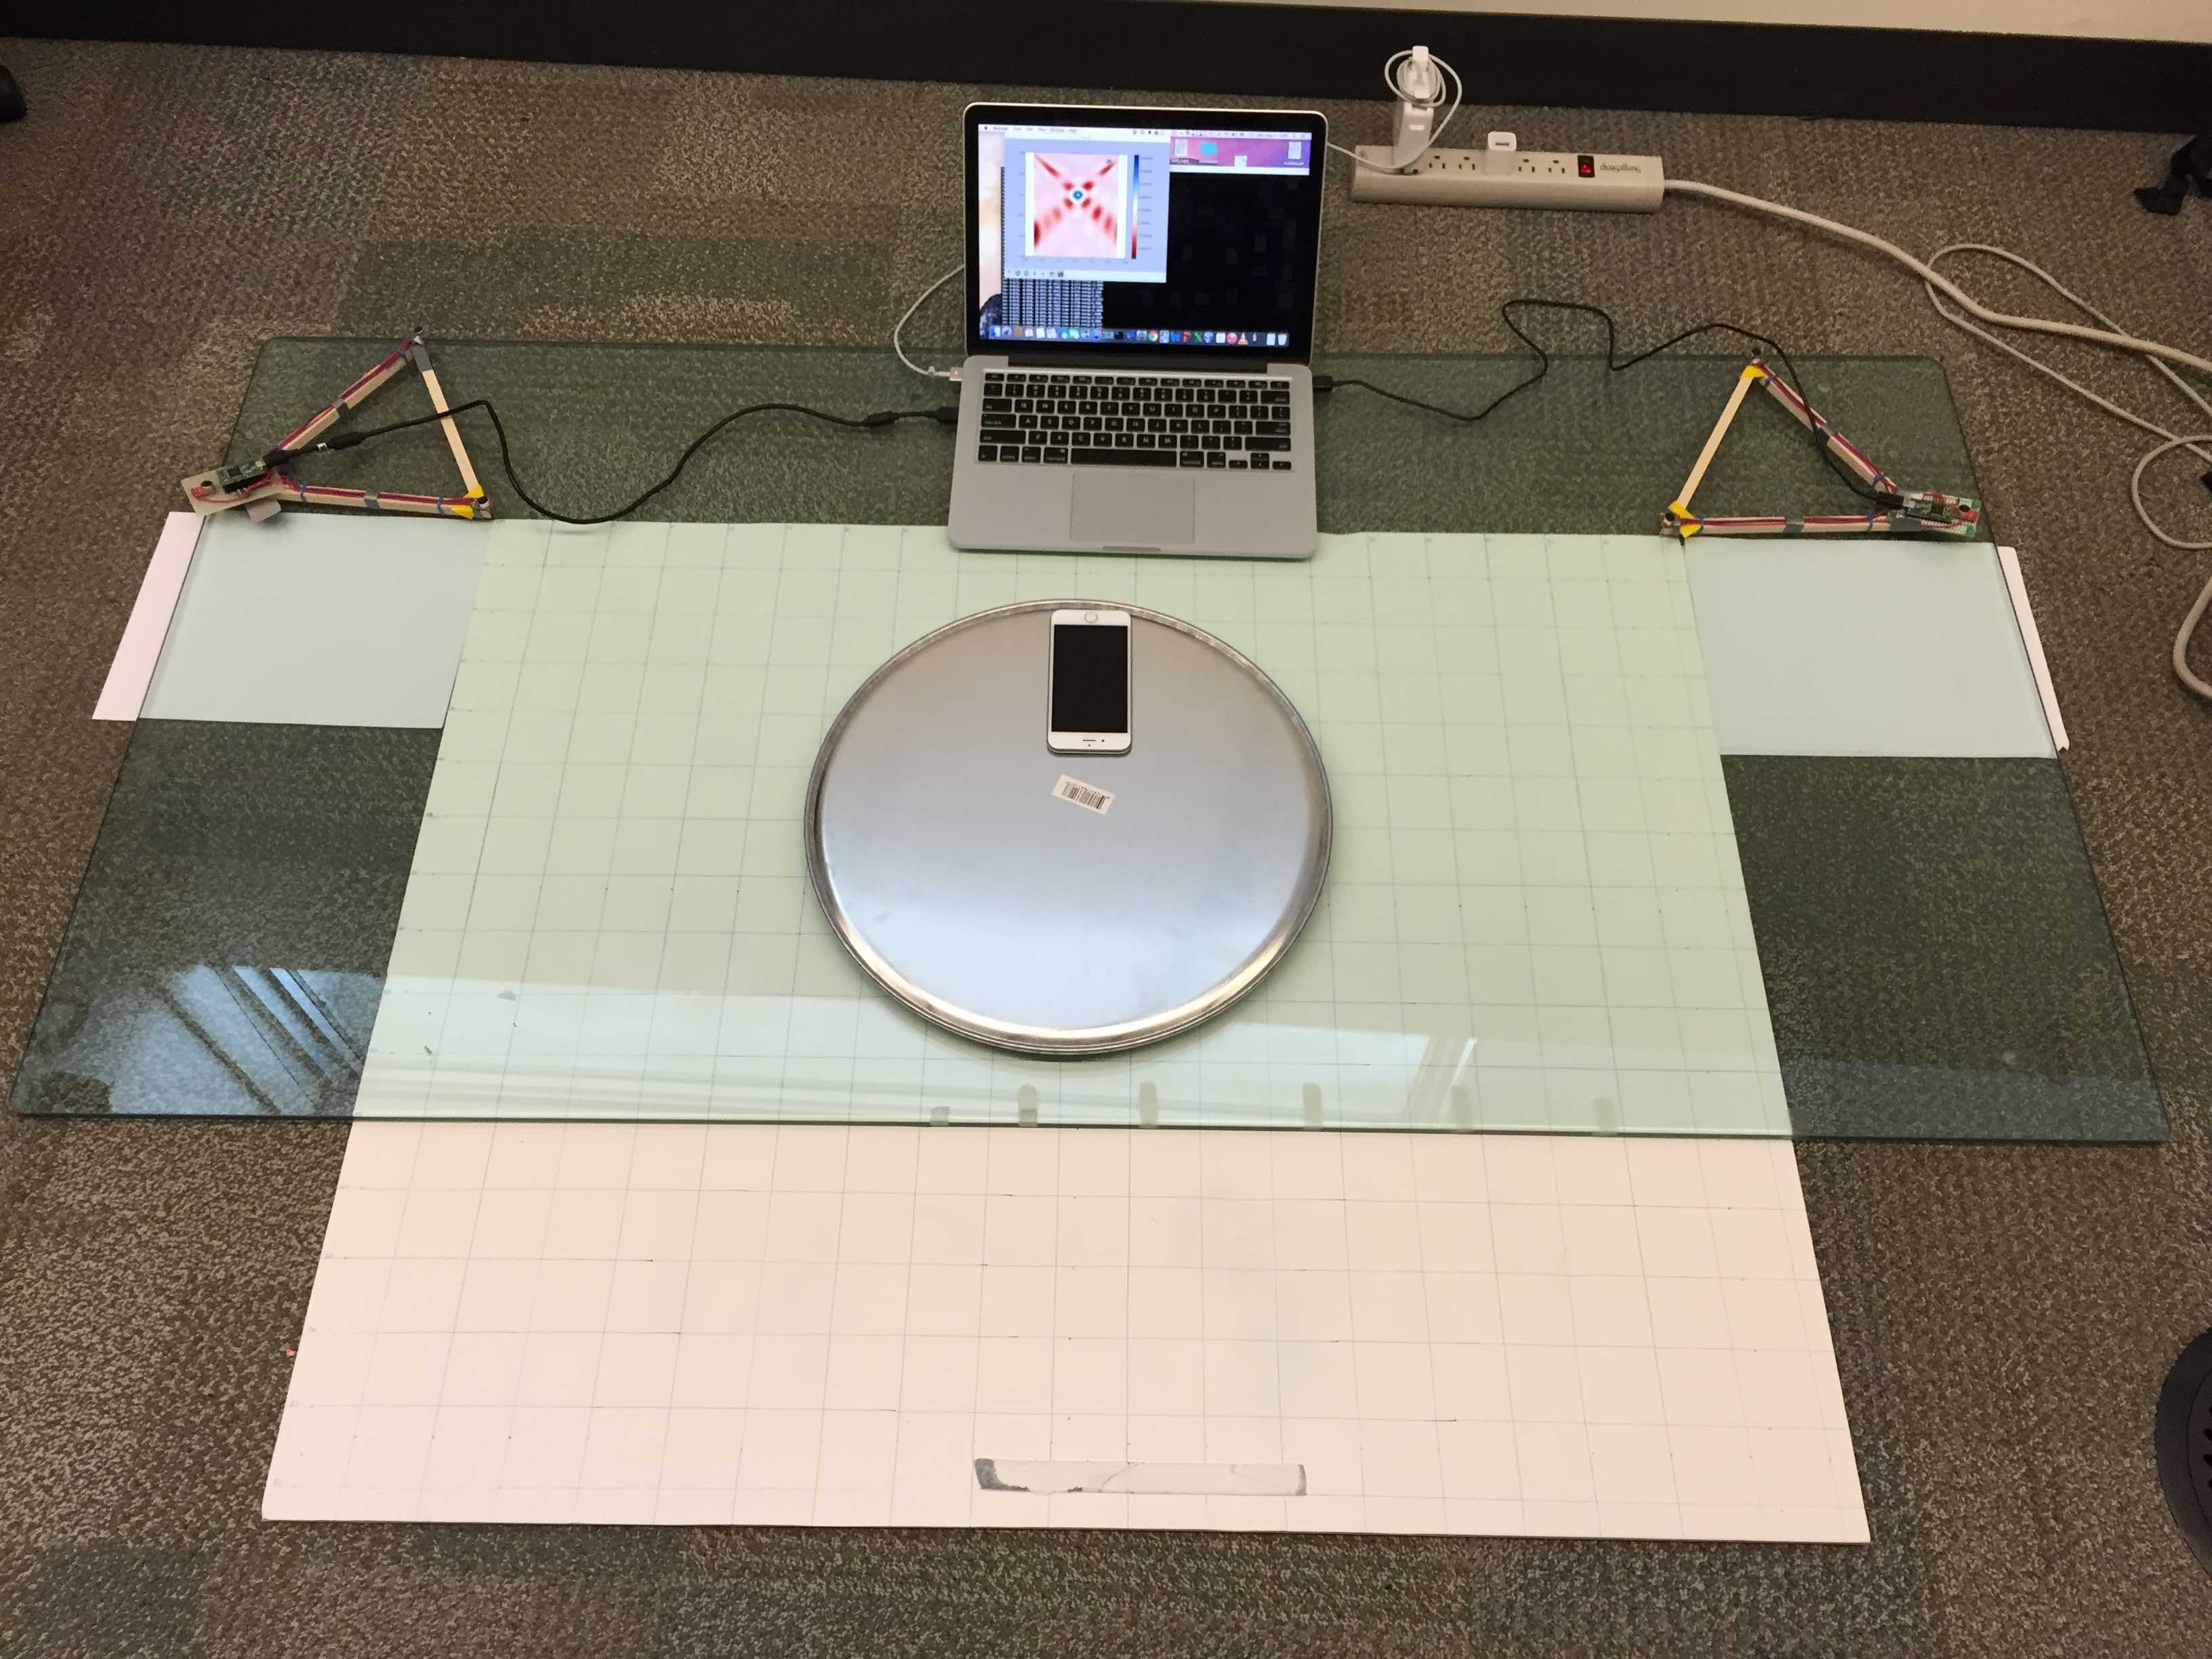
\includegraphics[width=\textwidth]{setup_rotating_disk.JPG}
  \end{subfigure}
  \caption{Setup for movement tracking evaluation}
  \label{fig:setup_circle}
\end{figure}


To test how well the system tracks movement, we mounted a rotating disk $40$ centimeters in diameter onto the grid at $(x=0$ cm$, y=-30$ cm$)$. Fig~\ref{fig:setup_circle} shows a picture of the setup. A sound source is placed on the edge of the rotating disk and the arrays track the sound source as it rotates in a circle. In this experiment we used GCC\_PHAT as the prefiltering for cross-correlation because in the point localization experiment we found out GCC\_PHAT gives the best result. In this experiment, we evaluated how accuracy changes with:
\begin{itemize}
\item window sizes 
\item audio sources
\item movement tracking filters
\item movement speeds
\end{itemize}

To test how localization accuracy varies with different window size of audio signal received, we conducted the experiment with audio signals with varying length from 1.02 ms to 12 ms.

To test how different sound sources impact localization quality, we conducted the experiments with three different sound sources:
\begin{description}%[\IEEEsetlabelwidth{long a label}\IEEEusemathlabelsep]

\item[White Noise] A recording of white noise. We expect GCC\_PHAT works best with white noise. The white noise is generated by sampling uniform randomly between $-1$ and $1$.

\item[Music A] A randomly picked music that has non-zero audio amplitude throughout the experiment period. \emph{Honest Eyes} by \emph{Black Tide} was the music used.

\item[Music B] A randomly picked music with intermittent low amplitude sections. \emph{Canon} was the music used.

\end{description} 

To test how the movement speed of sound source affects localization quality, each experiment was conducted at two different speeds:

\begin{description}
\item[Normal] An angular speed of $0.5$ rad/s was maintained, which translates to a linear speed of $10$ cm/s.
\item[Fast] An angular speed of $1.0$ rad/s was maintained, which translates to a linear speed of $20$ cm/s.
\end{description}

For each experiment conducted, two different movement filters were evaluated:
\begin{description}%[\IEEEsetlabelwidth{Very long label}\IEEEusemathlabelsep]
\item[Averaging filter] localization for past $0.5$ seconds were averaged and outputted as current estimate.
\item[Kalman filter] A 2nd order Kalman filter was used.
\end{description}

In the movement tracking experiments described above, we know the ground truth location of the circle, but not the exact location of the audio source at each moment during the movement. Therefore, the error is reported as the distance between the localized point to its closest point on the ground truth circle.
\clearpage

\section{Results}
\subsection{Point localization}
\begin{figure}[h!]
\centering
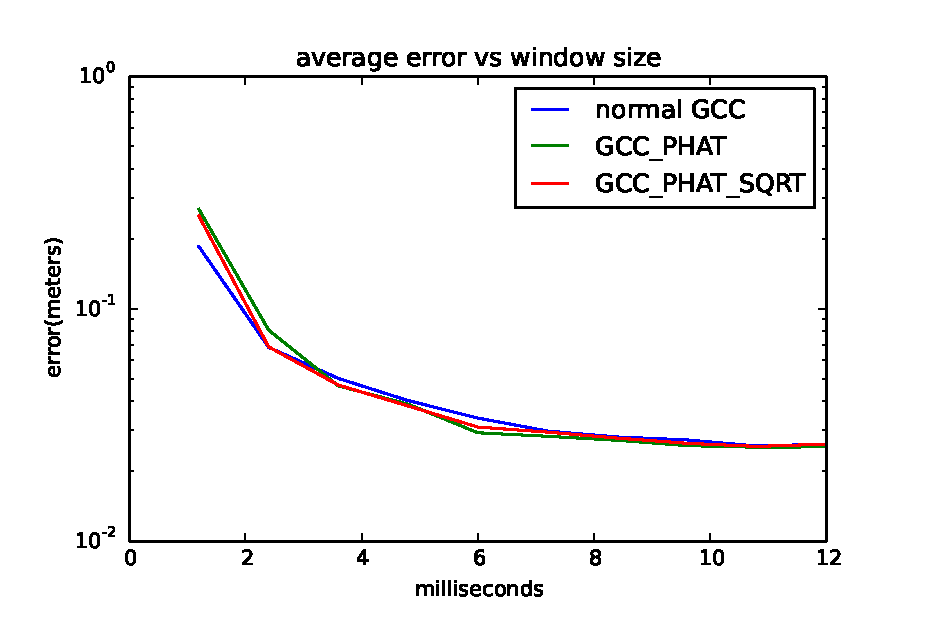
\includegraphics[width=1.0\textwidth]{average_error_window_size.eps}
\caption{Localization error versus window size}
\label{fig:accuracy_vs_window}
\end{figure}
To test how accuracy varies with window size, the algorithm is fed with microphone data of different lengths, and the result is shown in fig~\ref{fig:accuracy_vs_window}. The error decreases as window size increases and plateaus after the window size exceeds around $10$ millisecond. The lowest error achieved is $2.53$ centimeters, which occurred when the window size is set to 12 millisecond and when GCC\_PHAT is used for TDOA estimation. The performance differences among GCC, GCC\_PHAT and GCC\_PHAT\_SQRT is small.

\begin{figure}[h!]
\centering
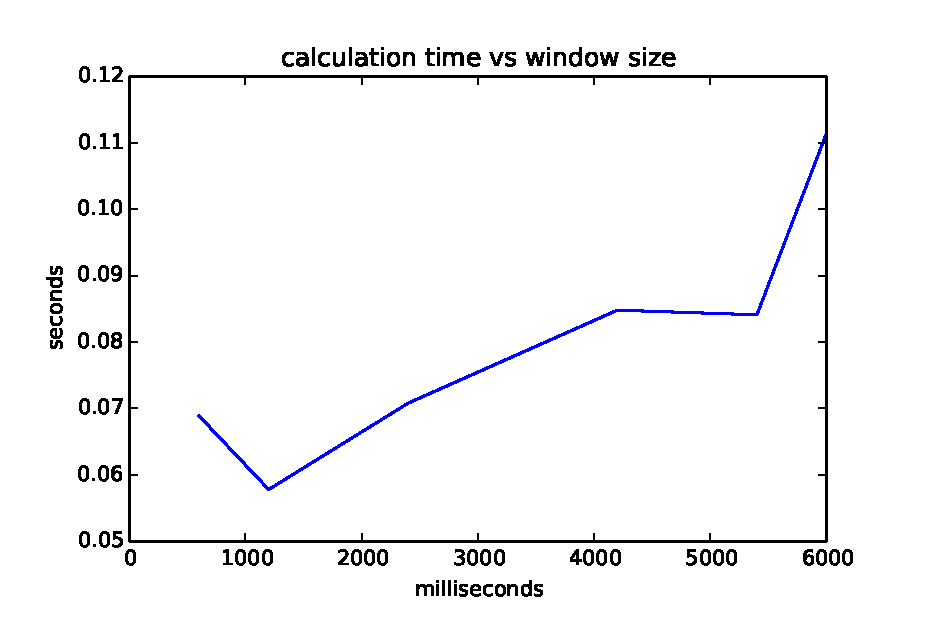
\includegraphics[width=1.0\textwidth]{calculation_time.eps}
\caption{Computation time versus window size}
\label{fig:speed_vs_window}
\end{figure}
As was mentioned before, although accuracy improves with the window size, computation time also increases with it. The part of calculation that depends on the window size is using cross correlation for TDOA estimation. Cross correlation can be calculated with Fast Fourier Transform (FFT) and the runtime is of order $O(N\log N)$. We measured how the computation time varied with window size and Figure~\ref{fig:speed_vs_window} shows the result. The runtime increases approximately linearly in the window size region of interest.

\begin{figure}[h!]
\centering
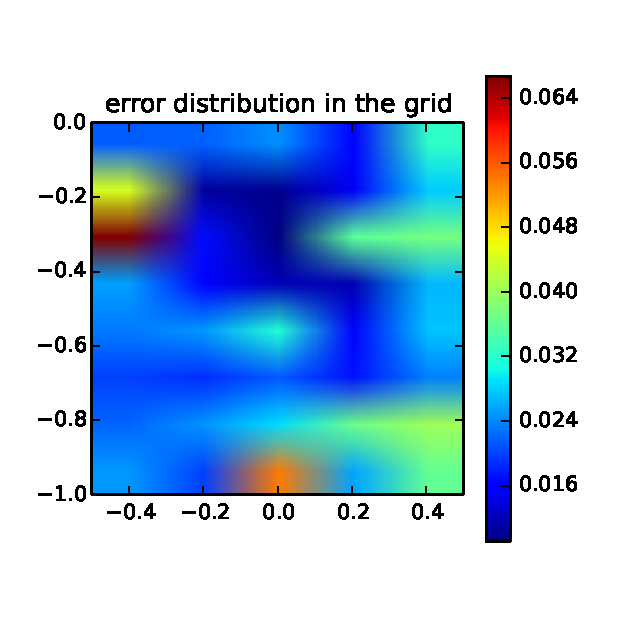
\includegraphics[width=1.0\textwidth]{error_distribution.eps}
\caption{error distribution in the grid. Arrays are placed at $(-0.5$ m$, 0$ m$)$ and $(0.5$ m$, 0$ m$)$}
\label{fig:error_distribution}
\end{figure}
We also calculated the localization error for each tested point in the grid. Figure~\ref{fig:error_distribution} shows the error distribution inside the grid. The error is below $3$ cm for most areas inside the grid. There is one error spike in the mid-left region and we contribute this to audio source misplacement because the error is fairly low and consistent around that spike.

\begin{figure}[h!]
\centering
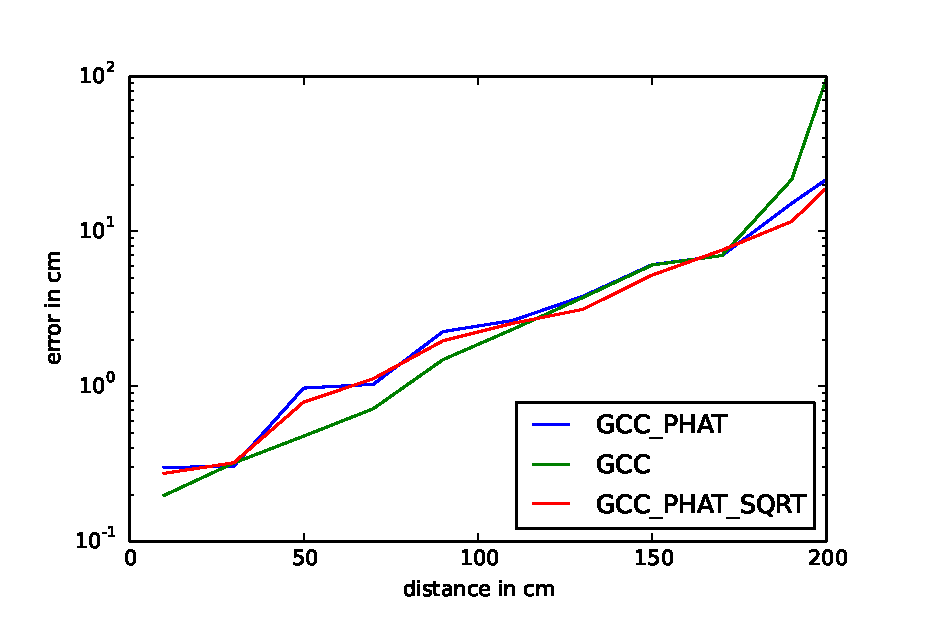
\includegraphics[width=1.0\textwidth]{error_along_y_axis.eps}
\caption{Localization error as the distance between the source and the microphone arrays increases. The source is placed on the $y$ axis.}
\label{fig:error_along_y}
\end{figure}
To test the limit of the system and to evaluate the accuracy when the source moves outside of the one meter by one meter region, we measured the localization error by placing the source at $10$ locations along $y$ axis ranging from $(0$ cm$, -10$ cm$)$ to $(0$ cm$, -200$ cm$)$. The result is presented in fig~\ref{fig:error_along_y}. The localization error is within $3$ cm when the source is within $100$ cm from the arrays. The error increases to about $5$ cm when the source distance increases to $150$ cm and the error exceeds $10$ cm after the source distance reaches $200$ cm.

\clearpage
\subsection{Movement tracking}
\begin{figure*}[h!]
\centering
  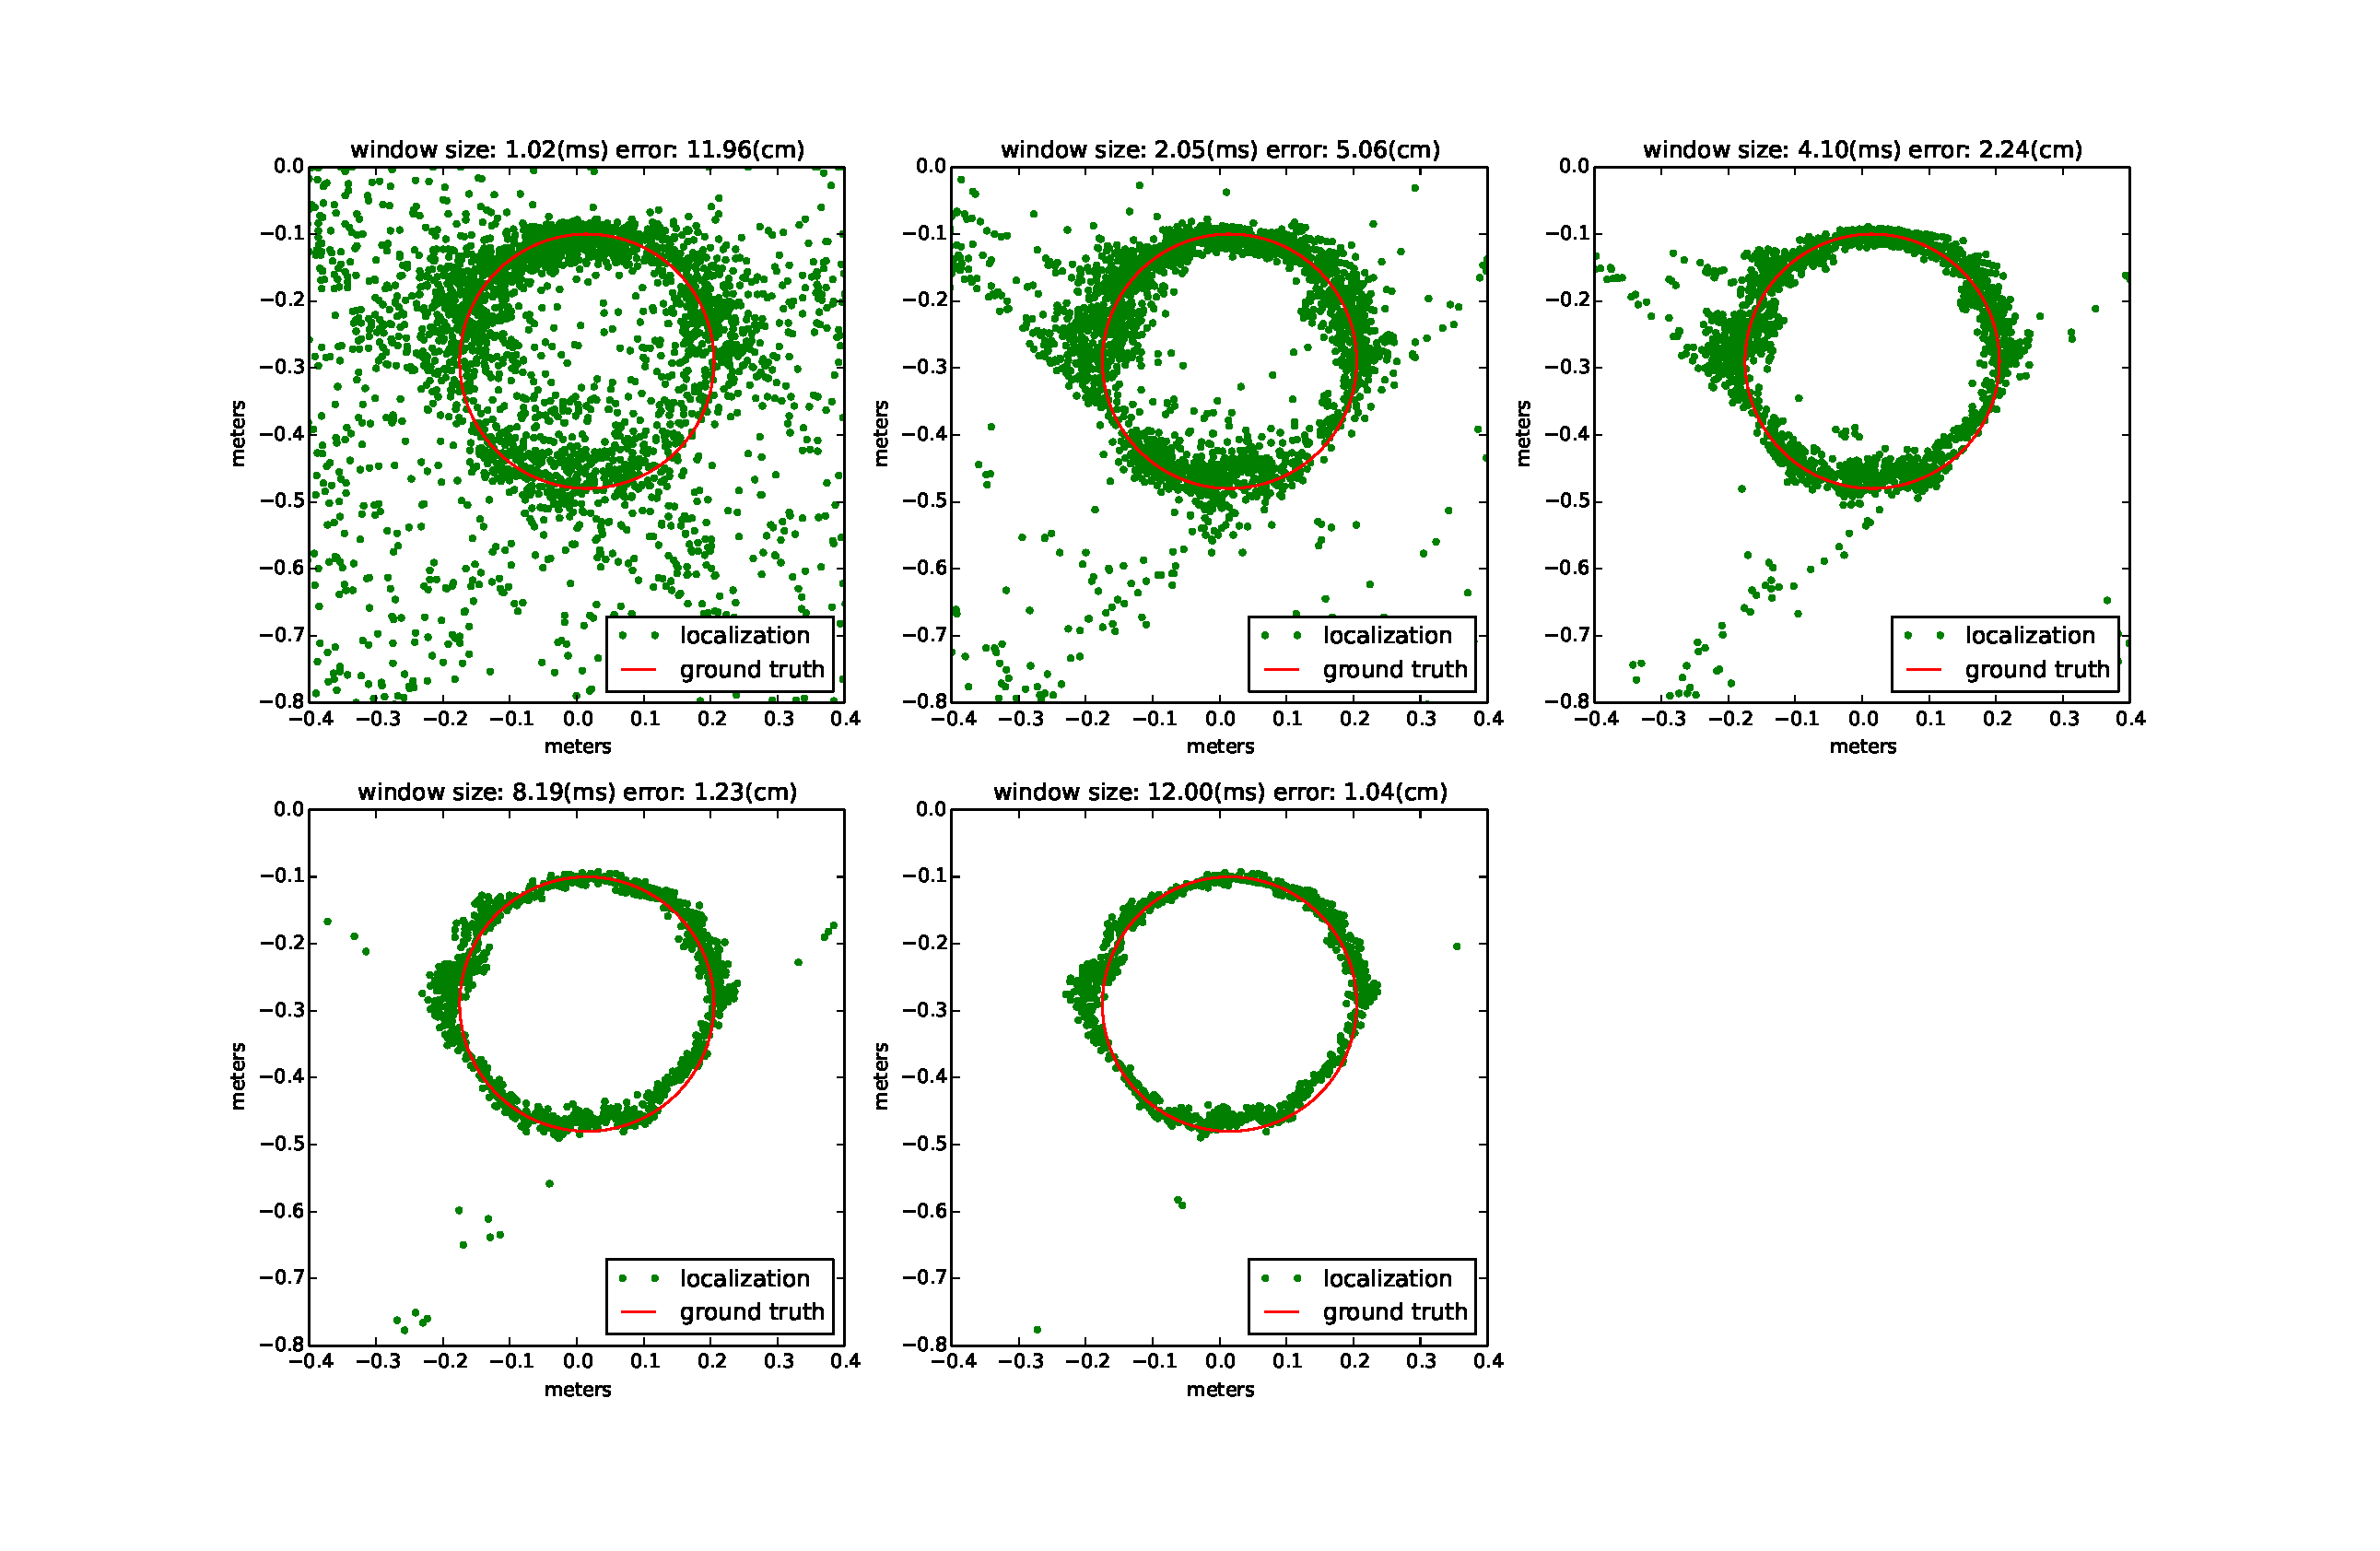
\includegraphics[width=\textwidth]{trace_window_size_movement.eps}
\caption{Localization quality versus window size}\label{fig:wn}
\label{fig:trace_win_circle}
\end{figure*}

\begin{figure}[h!]
\centering
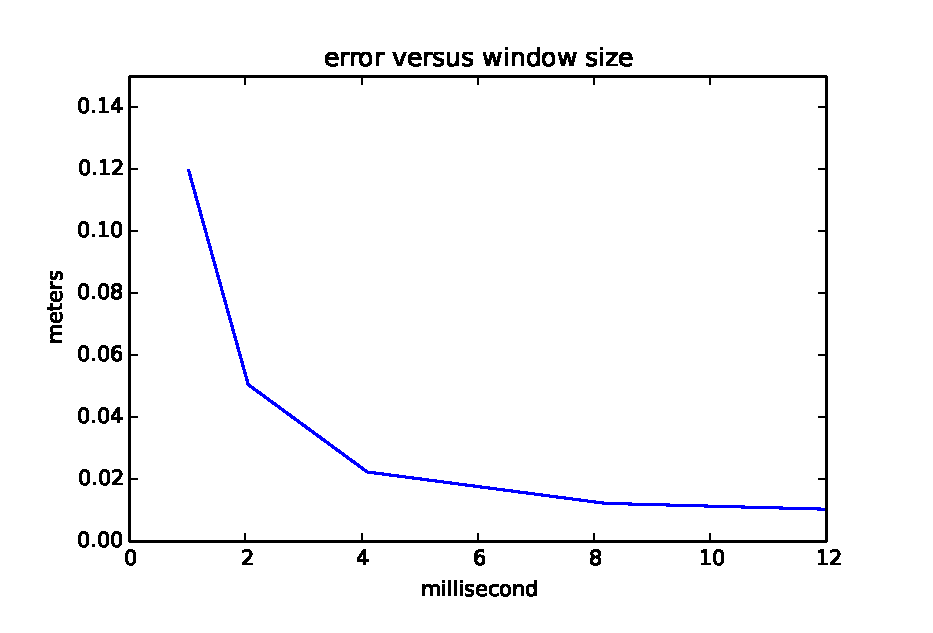
\includegraphics[width=1.0\textwidth]{error_window_size_movement.eps}
\caption{Localization error versus window size}
\label{fig:err_win_circle}
\end{figure}
Fig~\ref{fig:wn} gives an intuitive representation of how accuracy changes with window size. When window size is small ($1.02$ millisecond), the audio does not contain enough information to reliably estimate TDOA, which results in noisy localization. As window size increases, the TDOA estimation becomes more accurate and the localization converges to the shape of the ground truth circle. Fig~\ref{fig:err_win_circle} shows how the error changes with window size. The general trend is similar to that in point localization case. Error decreases as the window size increases and plateaus after it exceeds around $10$ milliseconds.

\begin{figure*}[h!]
\centering
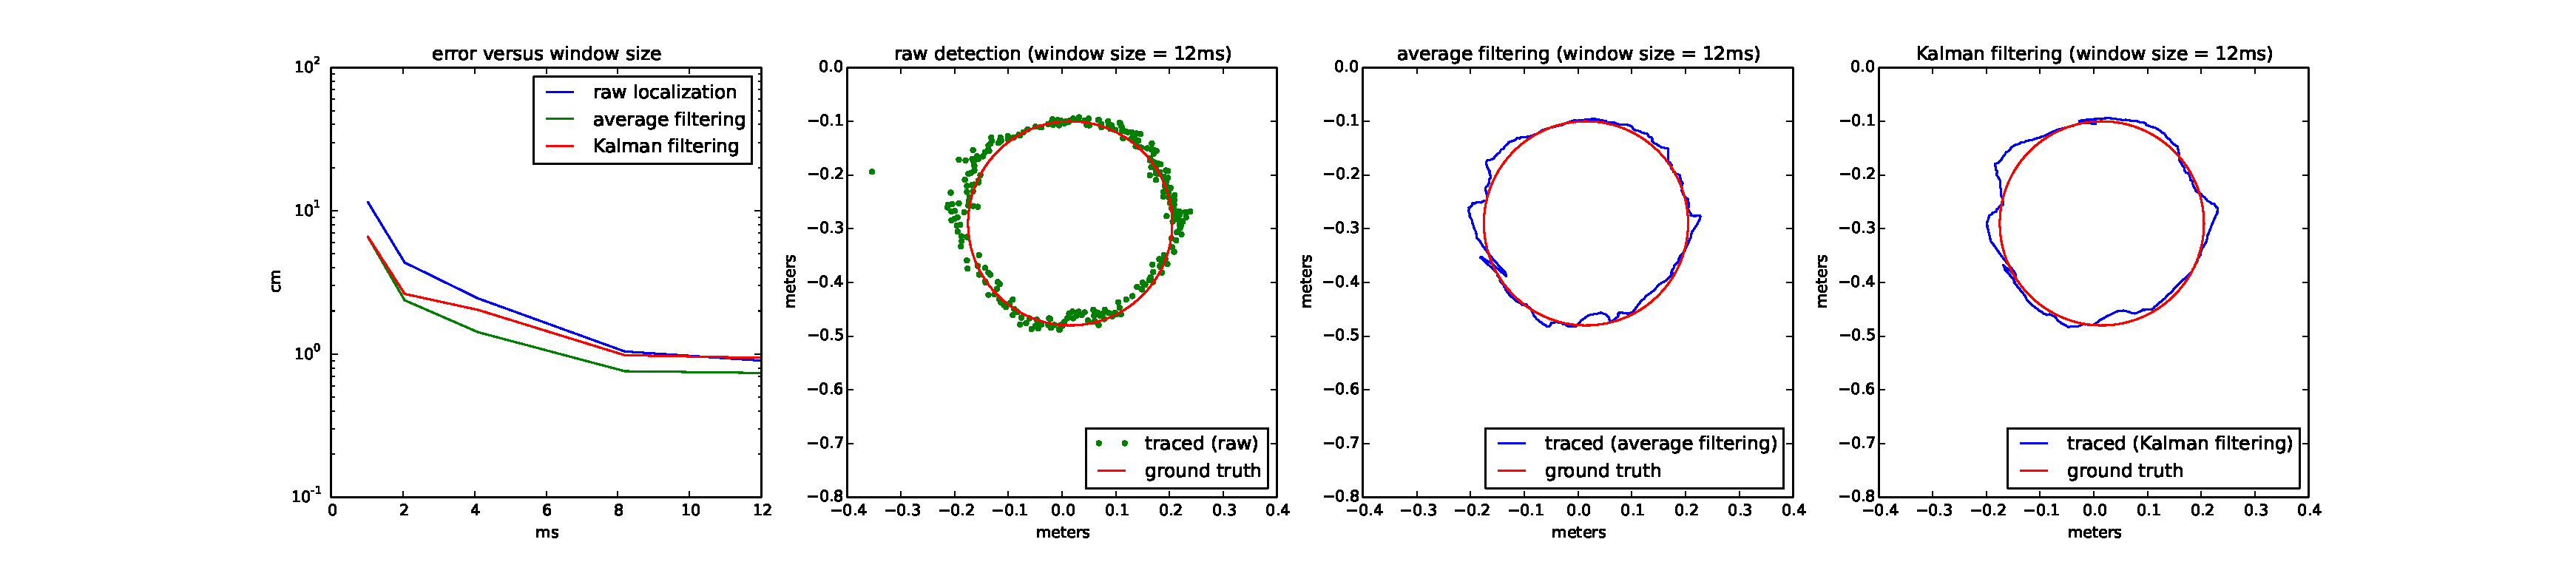
\includegraphics[width=1.0\textwidth]{trace_output_circle_wnn.eps}
\caption{white noise ($10$ cm per second)}
\label{fig:circle_wnn}
\end{figure*}

Fig~\ref{fig:circle_wnn} shows the result when white noise is used as the sound source and the source is rotated at $10$ cm per second. The top right plot in this figures shows the raw detection output with the ground truth circle overlayed on top. It shows that the array's raw output matches the underneath ground truth circle reasonably well. The average error between the localization output with its closest point on the ground truth circle is $0.9$ cm. The top left plot in the figure shows the average error with different movement filters applied as a function of window size. The error decreases as window size increases until the window size exceeds around $10$ ms. When the window size is $12$ cm, the localization accuracy is similar among raw output, Kalman filtering output and averaging filtering output. The bottom left plot shows the tracked movement for averaging filter and the bottom right filter shows the tracked movement for Kalman filtering. Kalman filtering result is smoother while the averaging tracking stays closer to the ground truth circle. Compared to the experiment in fig~\ref{fig:circle_wnf}, where the same sound source is played but rotated at a faster linear speed of $20$ cm per second, we find that the performance is equally good between these two movement speeds.

\begin{figure*}[h!]
\centering
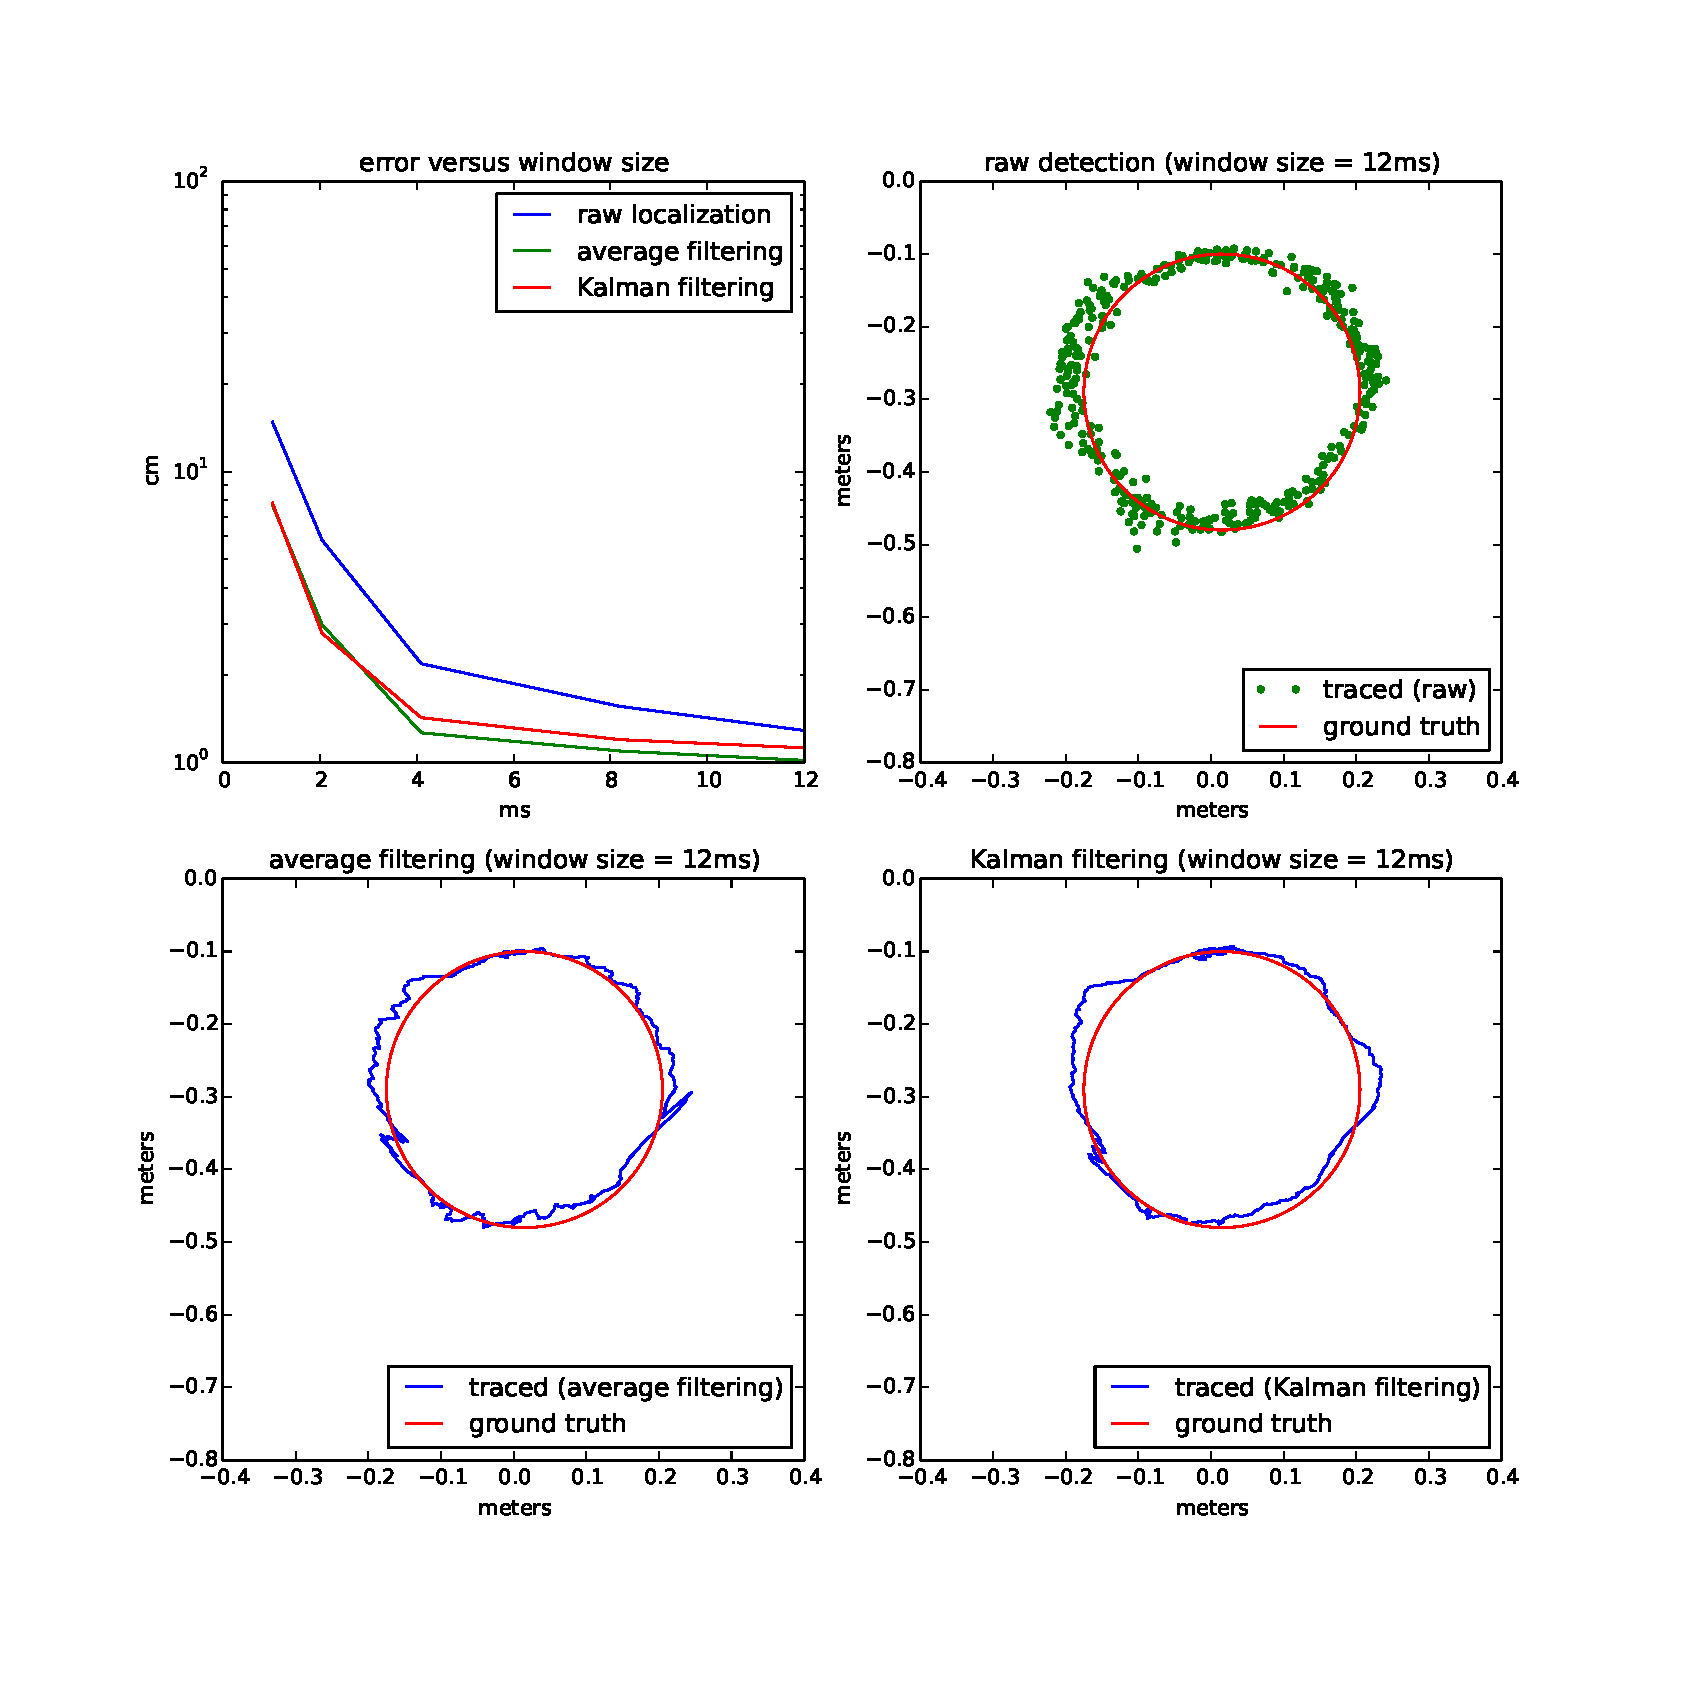
\includegraphics[width=1.0\textwidth]{trace_output_circle_man.eps}
\caption{music A ($10$ cm per second)}
\label{fig:circle_musican}
\end{figure*}

Fig~\ref{fig:circle_musican} shows the result when Music A is used as the sound source.  The top right plot shows that the array still tracks the movement well, but has a slightly larger deviation compared to that in fig~\ref{fig:circle_wnn} when white noise was used. The average localization error for Music A is $1.289$ cm. From the top left plot, it can be seen that the error still decreases with the window size. The performance improvement from raw output to Kalman filtering output is bigger than that with white noise (top left plot of fig~\ref{fig:circle_wnn}). Averaging filtering still produces lowest average error. Fig~\ref{fig:circle_musicaf} shows the result for the same sound source moved at twice the speed ($20$ cm per second). The average localization error at the faster speed is $1.291$ cm. Comparing the two experiments where music A was used as the sound source but with different movement speed, we find that the performance does not degrade as the movement speed increases from $10$ cm per second to $20$ cm per second. 

\begin{figure*}[h!]
\centering
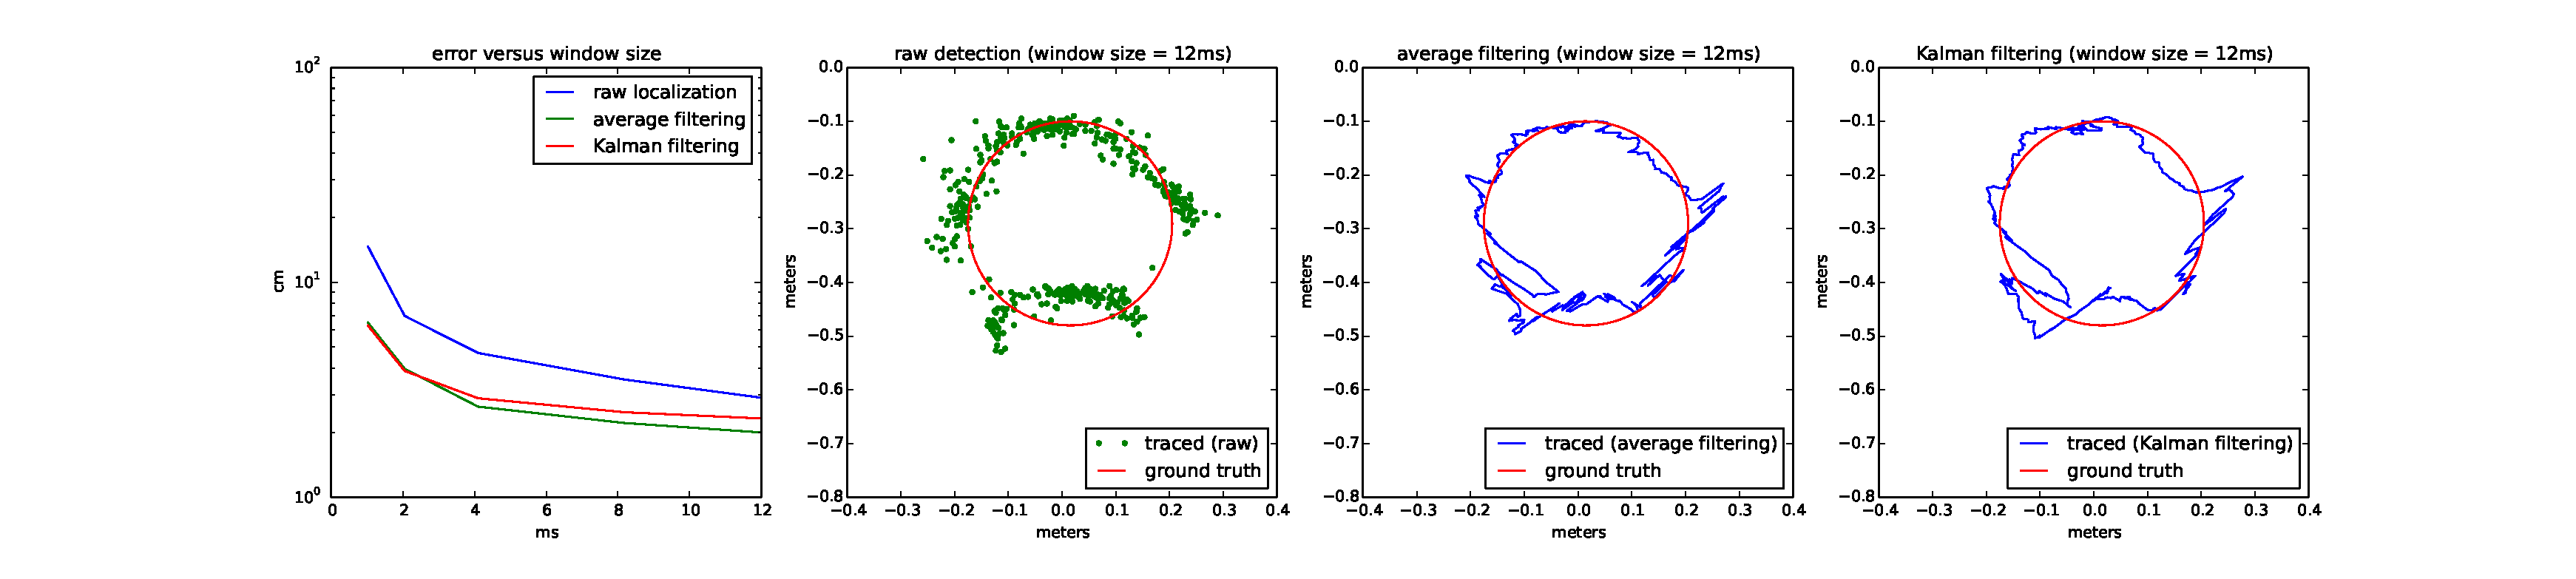
\includegraphics[width=1.0\textwidth]{trace_output_circle_mbn.eps}
\caption{music B ($10$ cm per second)}
\label{fig:circle_musicbn}
\end{figure*}

Fig~\ref{fig:circle_musicbn} shows the result when Music B is used as the sound source.  The low amplitude intervals in Music B affects the performance significantly. The average localization error is $2.9$ cm. The ``blank'' regions in the music can also be visually seen from the top right plot. The top left plot shows that the Kalman filtering still performs better than raw output. The performance improvement of Kalman filtering is similar to that with Music A. Averaging filtering produces lowest average error. Comparing to the faster movement experiment of the same sound source (shown in fig~\ref{fig:circle_musicbf}), we find that the localization error is similar between these two movement speeds.

\begin{figure*}[h!]
\centering
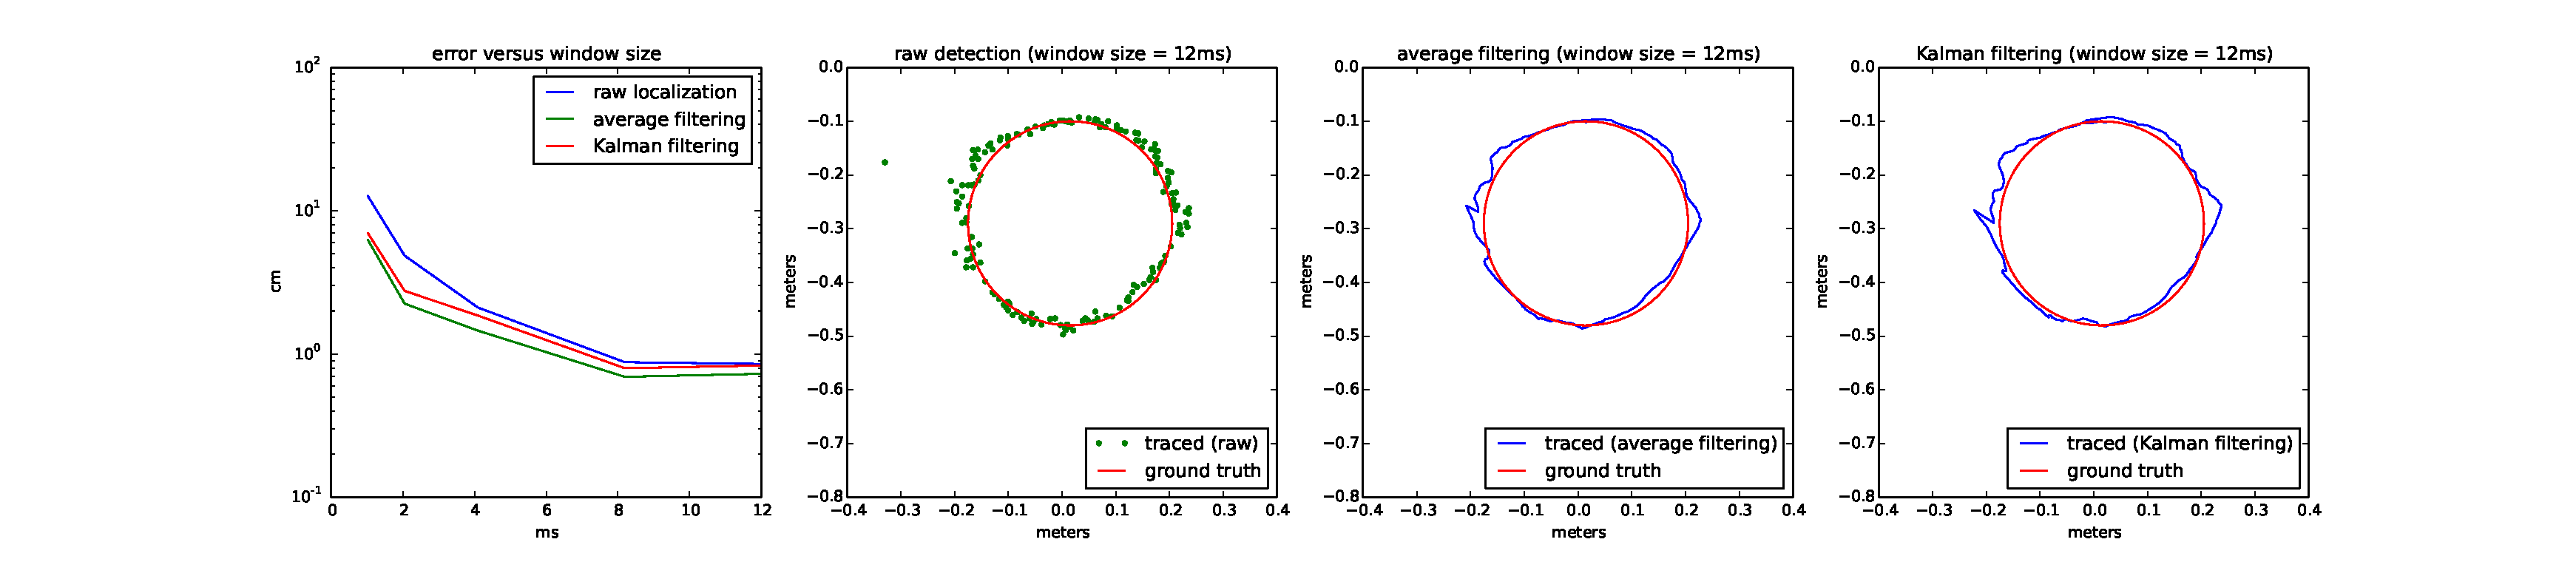
\includegraphics[width=1.0\textwidth]{trace_output_circle_wnf.eps}
\caption{white noise ($20$ cm per second)}
\label{fig:circle_wnf}
\end{figure*}

\begin{figure*}[h!]
\centering
  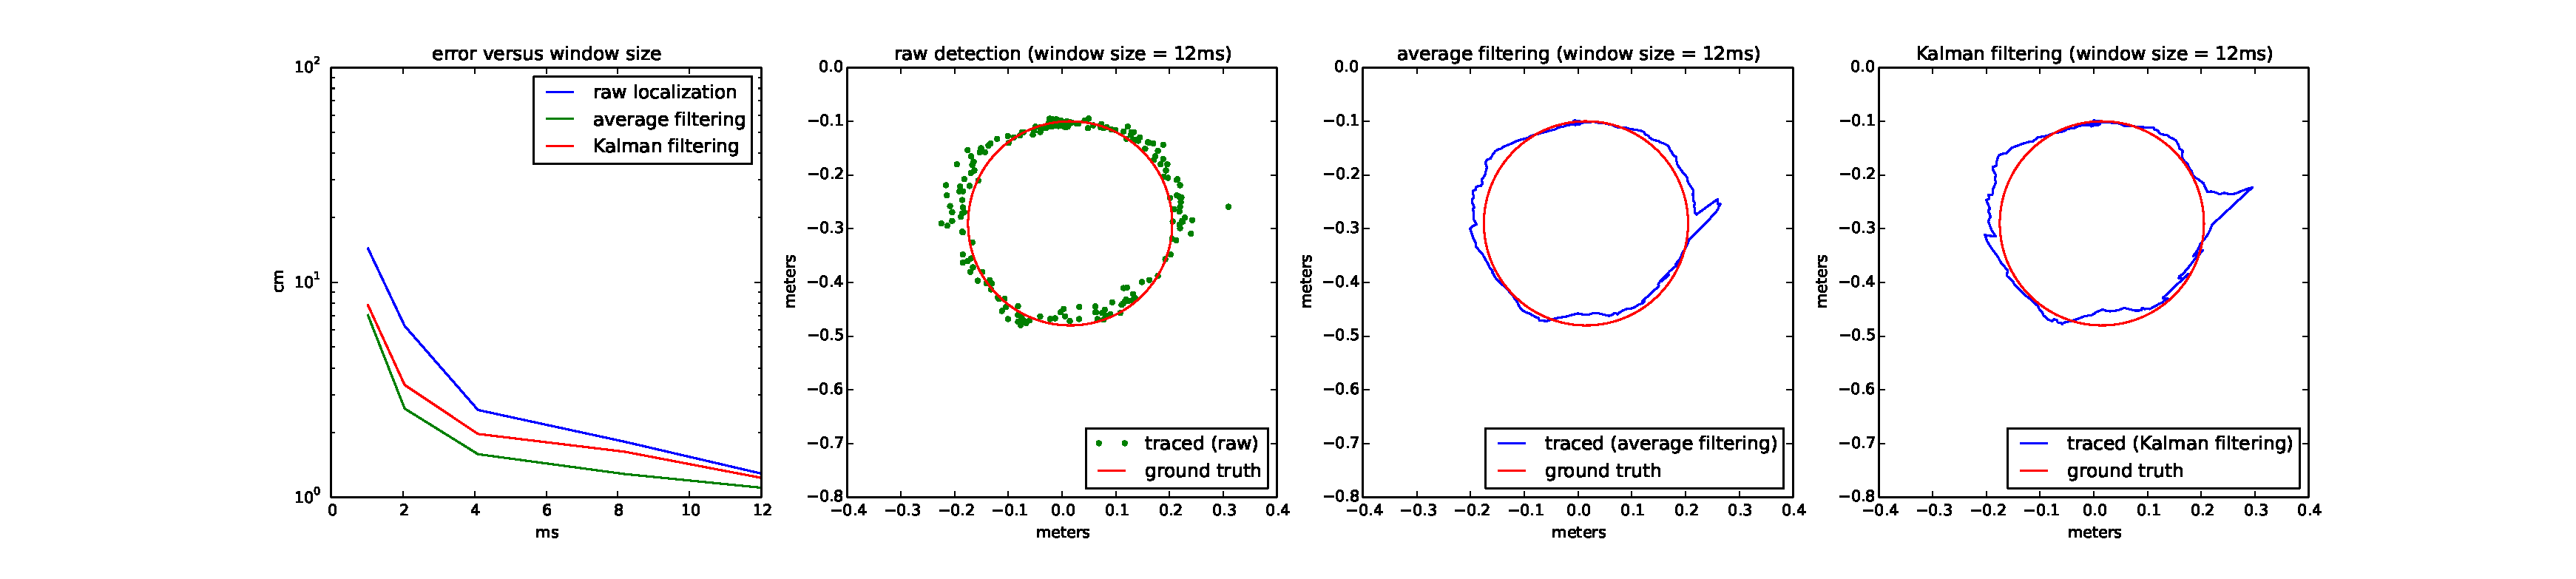
\includegraphics[width=1.0\textwidth]{trace_output_circle_maf.eps}
  \caption{music A ($20$ cm per second)}
  \label{fig:circle_musicaf}
\end{figure*}

\begin{figure*}[h!]
\centering
  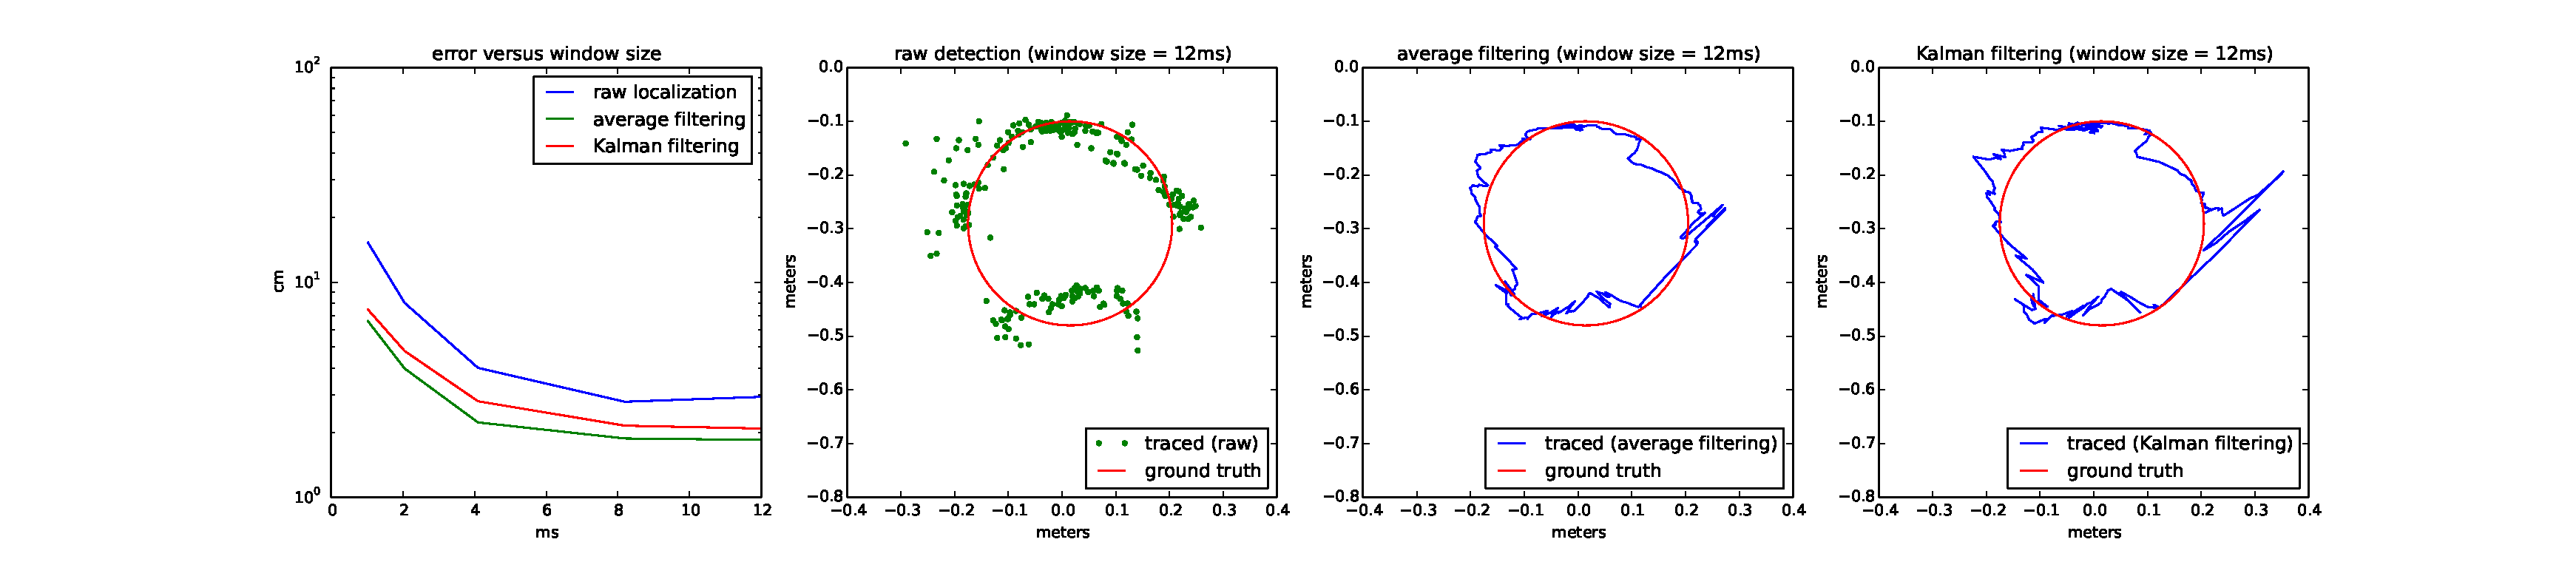
\includegraphics[width=1.0\textwidth]{trace_output_circle_mbf.eps}
  \caption{music B ($20$ cm per second)}
  \label{fig:circle_musicbf}
\end{figure*}

\subsection{Discussion}

Different prefiltering options produce very similar result. GCC\_PHAT gives slightly better accuracy, but the difference among unfiltered GCC, GCC\_PHAT and GCC\_PHAT\_SQRT is very small.

By comparing experiments at normal speed (fig~\ref{fig:circle_wnn} to \ref{fig:circle_musicbn}) with experiments at fast speed (fig~\ref{fig:circle_wnf} to~\ref{fig:circle_musicbf}), we find that the localization error does not increase when the movement speed increased from $10$ cm per second to $20$ cm per second.

When white noise is used as the audio source, Kalman filtering and raw localization produces very similar accuracy, and averaging filter gives slightly higher accuracy. However, when the audio source is changed to Music A or Music B, Kalman filtering produces better accuracy compared to raw detection, but Averaging filter still gives the best result. Looking at the smoothness of the movement path after applying different movement filters, it can be seen that raw detection has the most amount of jiggling. Kalman filter reduces the amount of jiggling from raw detection by combining past estimates with current estimates. Averaging filter has the least amount of jiggling. However, averaging filter averages detection outputs from past $0.5$ seconds, which makes the filtered output lag the real movement.

\begin{figure}[h!]
  \centering
  \begin{subfigure}[]{.48\textwidth}
    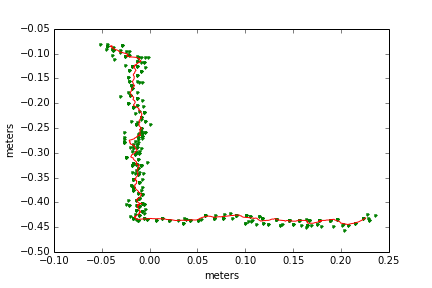
\includegraphics[width=\textwidth]{show_l.png}
    \caption{drawing letter `L'}
  \end{subfigure}
  \begin{subfigure}[]{.48\textwidth}
    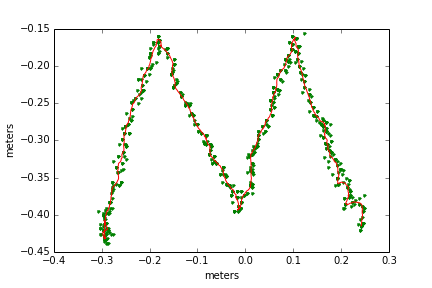
\includegraphics[width=\textwidth]{show_m.png}
    \caption{drawing letter `M'}
  \end{subfigure}

  \begin{subfigure}[]{.48\textwidth}
    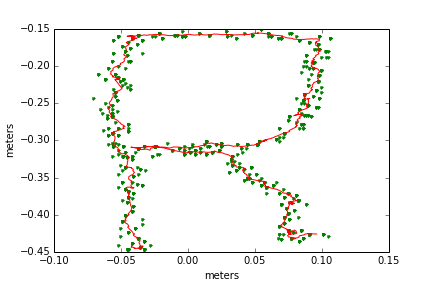
\includegraphics[width=\textwidth]{show_r.png}
    \caption{drawing letter `R'}
  \end{subfigure}
  \begin{subfigure}[]{.48\textwidth}
    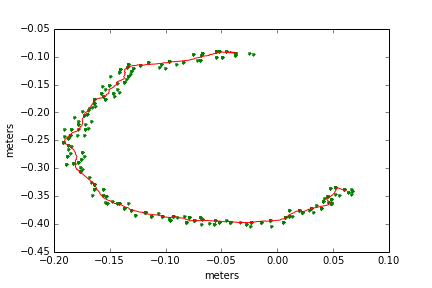
\includegraphics[width=\textwidth]{show_c.png}
    \caption{drawing letter `C'}
  \end{subfigure}
  \begin{subfigure}[]{.48\textwidth}
    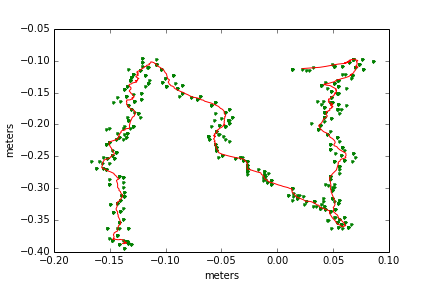
\includegraphics[width=\textwidth]{show_n.png}
    \caption{drawing letter `N'}
  \end{subfigure}
  \begin{subfigure}[]{.48\textwidth}
    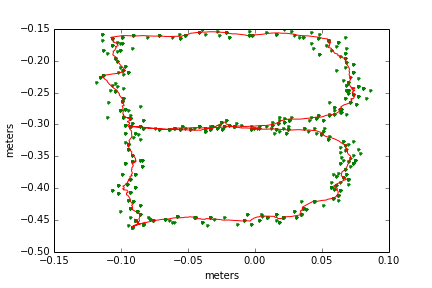
\includegraphics[width=\textwidth]{show_b.png}
    \caption{drawing letter `B'}
  \end{subfigure}
  \caption{Drawing letters. Green dots represent raw localization output and the red line is the output after averaging filtering.}
  \label{fig:show_case}
\end{figure}

In figure~\ref{fig:show_case}, a few examples of drawing letters with music are presented. Green dots on the plots represent the raw localization output and the red line shows the movement output with averaging filtering (window size of $0.5$ seconds is used). The demonstrated letters are drawn with free hand, without a track guiding the movement. The accuracy is reasonably good, and each letter can be easily recognized. There is a bit of jiggling in the tracked movement. Part of the jiggling can be attributed to the noise from system output, and the rest comes from the hand movement. 

\begin{figure}[h!]
\centering
  \begin{subfigure}[]{.48\textwidth}
    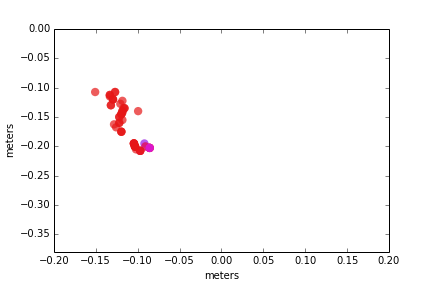
\includegraphics[width=\textwidth]{color_1.png}
    \caption{drawing a strip with maximum volume}
  \end{subfigure}
  \begin{subfigure}[]{.48\textwidth}
    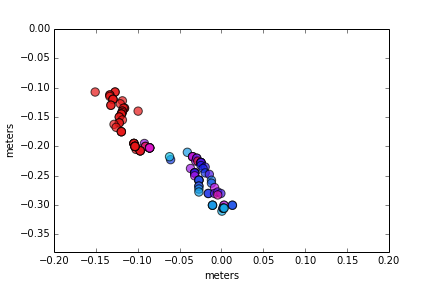
\includegraphics[width=\textwidth]{color_2.png}
    \caption{Drawing another strip with the volume decreased by $20\%$}
  \end{subfigure}
  \begin{subfigure}[]{.48\textwidth}
    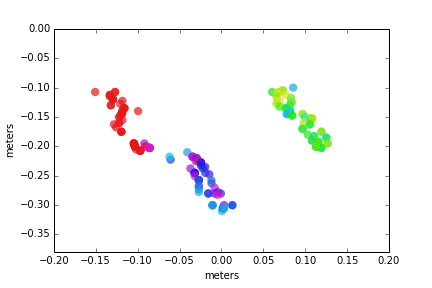
\includegraphics[width=\textwidth]{color_3.png}
    \caption{Drawing a third strip with the volume decreased by an additional $20\%$}
  \end{subfigure}
\end{figure}

\begin{figure}[h!]
\centering
  \begin{subfigure}[]{1.0\textwidth}
    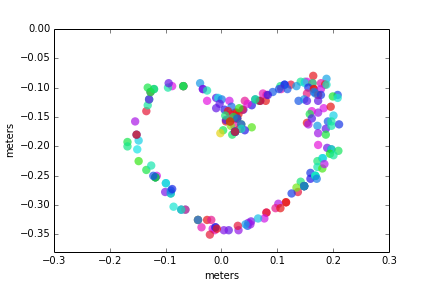
\includegraphics[width=\textwidth]{color_4.png}
    \caption{Painting a heart shape with free hand. The color of the heart changes with the volume of the song.}
  \end{subfigure}
\end{figure}
